\documentclass[simple,a4paper,14pt,ukrainian,utf8]{eskdtext}

\usepackage[T2A]{fontenc}
\usepackage{amsfonts,amssymb,amsmath,mathtext,cite,float}
\usepackage{setspace}
\usepackage{listings}
\usepackage{indentfirst} % отделять первую строку раздела абзацным отступом тоже
\usepackage[nottoc]{tocbibind}
\usepackage[toc,page]{appendix}
\usepackage{lscape}

\newcommand{\abs}[1]{\lvert#1\rvert} % vector module

\usepackage{geometry} % Меняем поля страницы
\geometry{left=25mm}% левое поле
\geometry{right=1.5cm}% правое поле
\geometry{top=1cm}% верхнее поле
\geometry{bottom=25mm}% нижнее поле

\setcounter{tocdepth}{3}

\renewcommand{\appendixtocname}{Додатки}
\renewcommand{\appendixname}{Додатки}
\renewcommand{\appendixpagename}{Додатки}

\onehalfspacing % полуторный интервал для всего текста
% или \singlespacing % одиночный интервал для всего текста
% или \doublespacing % двойной интервал для всего текста
% или \setstretch{множитель} % произвольный интервал

\DeclareUnicodeCharacter{00A0}{ }

\begin{document}

  \ESKDthisStyle{empty}

  \begin{titlepage}
    \fontsize{10pt}{12pt}\selectfont
    \newpage

    \begin{center}
        Міністерство освіти і науки України \\
        \vspace{1em}
        Житомирський Державний Технологічний Університет \\*
    \end{center}

    \vspace{8em}

    \flushright{Кафедра ПЗС}
    \vspace{1em}
    \flushright{Група ПІ-39М}

    \vspace{8em}

    \begin{center}
        \Large Пояснювальна записка \\ до випускної роботи на тему:
    \end{center}

    \vspace{2.5em}

    \begin{center}
        \Large{\textbf{побудова тривимірної регіональної мапи за допомогою мобільних GPS-пристроїв}}
    \end{center}

    \vspace{6em}

    \begin{flushleft}
        Студент \hrulefill А. Г. Шубович \\

        \vspace{1.5em}

        Керівник роботи \hrulefill А. М. Ковальчук \\

        \vspace{1.5em}

        Завідувач кафедри \hrulefill А. В. Панішев \\
    \end{flushleft}

    \vspace{\fill}

    \begin{center}
        Житомир 2014 р.
    \end{center}

  \end{titlepage}

\newpage

\begingroup
    \ESKDthisStyle{formII}

    \begin{abstract}
        В рамках даної випускної роботи розроблено систему створення тривимірної регіональної мапи за допомогою мобільних GPS-пристроїв. Система складається з двох частин:
        \begin{enumerate}
        	\item \textit{мобільний агент}, котрий зчитує дані з GPS-приймача та/або гіродатчиків і зберігає їх у файл
        	\item \textit{рендерер}, котрий відображає зчитані дані у вигляді тривимірної поверхні та дозволяє переглядати цю поверхню з різних ракурсів
        \end{enumerate}
        
        Було досліджено різні протоколи зберігання даних, зібраних з GPS-приймачів та способи візуалізації гео-даних.
         
        Проект розроблений з використанням мов програмування Java та C++, бібліотеки Qt та платформ Linux та Android.  Мобільний агент працює під керуванням ОС Android. Рендерер може працювати як в оточенні ОС Linux, так і в ОС Windows. Розробка мобільних агентів для спеціалізованих систем наразі триває.

    \vspace{10mm}
    
    \begin{center}
        \textbf{Abstract}    
    \end{center}
    
    	As a part of this work, a complex software system was created. System consists of two main parts:
    	\begin{enumerate}
    		\item \textit{mobile agent}, who reads GPS data and stores it in a file
    		\item \textit{renderer}, who displays the data being read as a three-dimensional surface and allows user to view that surface from different perspectives
    	\end{enumerate}
    	
		Different geo-data storage protocols and geo-data graphic representation methods were inspected as well.
    	
		Project was done using Java and C++ programming languages, Qt libraries, Linux and Android platforms. Mobile agent works under Android OS. Renderer is able to be run under Linux or Windows operating systems. Mobile agents for different task-specific platforms are still being developed.

        \normalsize
        \newpage
    \end{abstract}
\endgroup

\tableofcontents

\newpage

  \newpage
  \section*{Вступ}
  \addcontentsline{toc}{section}{Вступ}

    З нещодавнім масовим впровадженням смартфонів їх використання у повсякденному житті стало нормою для пересічної людини. Область застосування та можливості смартфонів дуже широкі - від читання книжок до тривимірних іграшок та відео-конференцій. Однією дуже корисною функцією сучасних смартфонів є підтримка GPS-навігації. Картографічні та геолокаційні сервіси активно впроваджують соціальну складову. Наприклад, спеціальна організація \textbf{Open Street Map \cite{website:osm}} довірила своїм користувачам редагування мапи світу. Все більш потужними стають і програми навігації, що підтримуються смартфонами і розширюються рамки області застосування цих мобільних пристроїв.

    Не так давно, за допомогою OSM, з’явився термін \textit{маппер}. Це - людина, котра подорожуючи світом, прокладає маршрути та зберігає їх у своєму GPS-пристрої. Після того, як маппер проклав кілька доріг, він завантажує дані на сервери OSM, після чого прокладені ним шляхи з’являються на світовій мапі. І вже за кілька хвилин ці зміни доступні всім користувачам мап OSM.
    
    Немало чим успіх OSM завдячує і розвитку операційної системи Android та смартфонів як популярної мобільної платформи. Завдяки величезній популярності даної ОС, стало можливим поширення мобільних додатків, котрі дозволяють орієнтуватись на місцевості та знаходити шлях до пункту призначення з поточної позиції. Це особливо корисна функція для людей, котрі вперше знаходяться в іншому місті, країні чи просто намагаються знайти певне місце на мапі.
    
    Чимало існує і програм для виконання подібних функцій. Найбільш відомими з них є Яндекс.Карты, Google Maps, OSMAnd, MapWithMe. Але у багатьої випадках, непросто уявити собі вірний маршрут чи обрати більш зручний шлях. Наприклад, у гірській місцевості, шлях між двома точками, який програма вказала як "найкоротший", може зайняти чимало часу через простий факт того, що подібні програми не враховують перепади висот на маршруті. Більшість з таких програм використовують для визначення відстані між двома точками у форматі \textbf{(lat, lng)} \textit{(широта, довгота)} формулу \textbf{Great Circle Distance \cite{website:great_circle_distance}}, яка приймає Землю за ідеальну кулю. Це дає змогу прискорити роботу пошукового алгоритму та зменшити навантаження на процесор, але дає менш точні результати.
    
    Розроблена в рамках даної роботи система чимось нагадує систему OSM та мапперів - мобільні агенти, що запускаються на ОС Android, прокладають шлях на основі даних, зчитаних з вбудованого в смартфон GPS-приймача\cite{website:gps_receiver}. Після цього, маппер передає файл, отриманий в результаті роботи програми, на обробку рендереру, котрий і відображає пройдений маппером шлях у вигляді тривимірної поверхні.
    
    Перегляд маршруту в такому форматі значно поліпшує сприйняття його, дозволяє більш ретельно вивчити всі його складнощі, порівняти з іншими, можливо, більш пологими дорогами.

\newpage \section{Технічне завдання}

    Розробити систему збору та відображення гео-позиційних даних про шляхи регіону.

    \begin{enumerate}
        \item Дослідити апаратні можливості платформ з GPS-приймачами
        \item Визначити та проаналізувати наявні формати збереження гео-даних
        \item Порівняти технології побудови та відображення тривимірних фігур
        \item Розробити мобільний агент для ОС Android
        \item Створити рендерер з керованим оглядом поверхні дороги
        \item Провести аналіз та тестування роботи системи в реальному житті
    \end{enumerate}

\newpage \section{Постановка задачі та аналіз шляхів її вирішення}

    \subsection{Пристрої з підтримкою GPS-приймача}
    
    Усі GPS-пристрої поділяються на \textit{професійні} та \textit{приймачі широкого застосування}.
	
	Професійні GPS-приймачі можна розділити на дві категорії:
    
    \begin{enumerate}
    	\item \textbf{геодезичні приймачі} - пристрої для геодезичних робіт у польових умовах
    	\item \textbf{приймачі ГІС-класу} - такі собі кишенькові портативні комп’ютери з вмонтованим GPS-приймачем
    \end{enumerate}
    
    GPS-приймачі для широкої цільової аудиторії поділяються на два види пристроїв навігації:
    
    \begin{enumerate}
    	\item \textbf{GPS-навігатори}, основна функція котрих - прийом та обробка сигналу гео-позиціювання зі супутників
    	\item \textbf{пристрої, що містять GPS-приймач}, де навігація та гео-локація не є основними цілями використання цих пристроїв
    \end{enumerate}
    
    Пристрої відрізняються якістю виготовлення компонентів (особливо антенн), програмним забезпеченням, режимами роботи, робочими діапазонами частот, алгоритмами подавлення інтерференційних залежностей, сонячної активності, системами навігації, терміном роботи від одного заряду акумулятора та, звісно ж, вартістю.

    Логічно було б припустити, що в якості платформи для мобільних агентів краще використати саме GPS-навігатори. Але моделей їх існує безліч, кожна з яких має свої особливості та інструментарій для розробки. 
    
    З іншого ж боку, моделей смартфонів на основі ОС Android чи iOS з вбудованим GPS-приймачем хоч і багато, зате особливості роботи та інструментарій для розробників у таких пристроїв стандартизовані. До того ж, вони значно більш поширені серед звичайних людей.
    
    Саме тому з метою збільшення цільової аудиторії мапперів було вирішено взяти за основу смартфони під керуванням ОС Android.

    \subsection{Формати GPS-даних}
    
    В якості формату спілкування GPS-приймача та різноманітних засобів обробки гео-даних (як програмних так і апаратних) використовуються варіації стандарту NMEA (\textit{National Marine Electronics Association}).
    
    Існує дві основних версії цього стандарту:
    
    \begin{enumerate}
    	\item \textbf{NMEA 0183 \cite{website:nmea_0183}}, який використовується у більшості не спеціалізованих програмних та апаратних засобів
    	\item \textbf{NMEA 2000 \cite{website:nmea_2000}}, який використовується у мережі подібних між собою пристроїв у морській та залізничній інфраструктурах
    \end{enumerate}
    
    Дані у форматі NMEA - це послідовність спеціальним чином відформатованих рядків. Кожен рядок даних у форматі NMEA 0183 має наступний вигляд:
    
    \begin{enumerate}
    	\item \textbf{символ \$}
		\item \textbf{ідентифікатор повідомлення} - дві літери, що визначають джерело сигналу та три літери, що визначають вміст рядка (тип даних)
		\item \textbf{дані} - список полів, розділених комами
		\item \textbf{CRLF} - кінець рядка
    \end{enumerate}
    
    В даній роботі було використано два типи рядків - \textbf{GPRMC} (Recommended Minimum sentence C), дані про поточне гео-розташування приймача та \textbf{PGRMZ} - дані про поточну висоту над рівнем моря у поточному гео-розташуванні приймача. Цих даних достатньо для побудови цілком відповідної реальності тривимірної поверхні пройденого шляху.

	\newpage
	
    \subsection{Відтворення шляху на мапі}
    
    З метою перевірки роботи алгоритму дешифрування даних, записаних мобільним агентом, було створено HTML-сторінку, за допомогою якої можна перевірити достовірність та точність даних.
    
    Сторінка використовує бібліотеку \textbf{leaflet} для керування відображенням мапи та маркерів на мапі. Для дешифрації рядків даних у форматі NMEA-0183, отриманих під час роботи мобільного агента, використовується невеликий скрипт мовою програмування \textbf{JavaScript}.
    
    У браузері набір даних, зібраних за допомогою спеціально облаштованого транспортного засобу, виглядає так:
    
    \vspace{3em}
    
    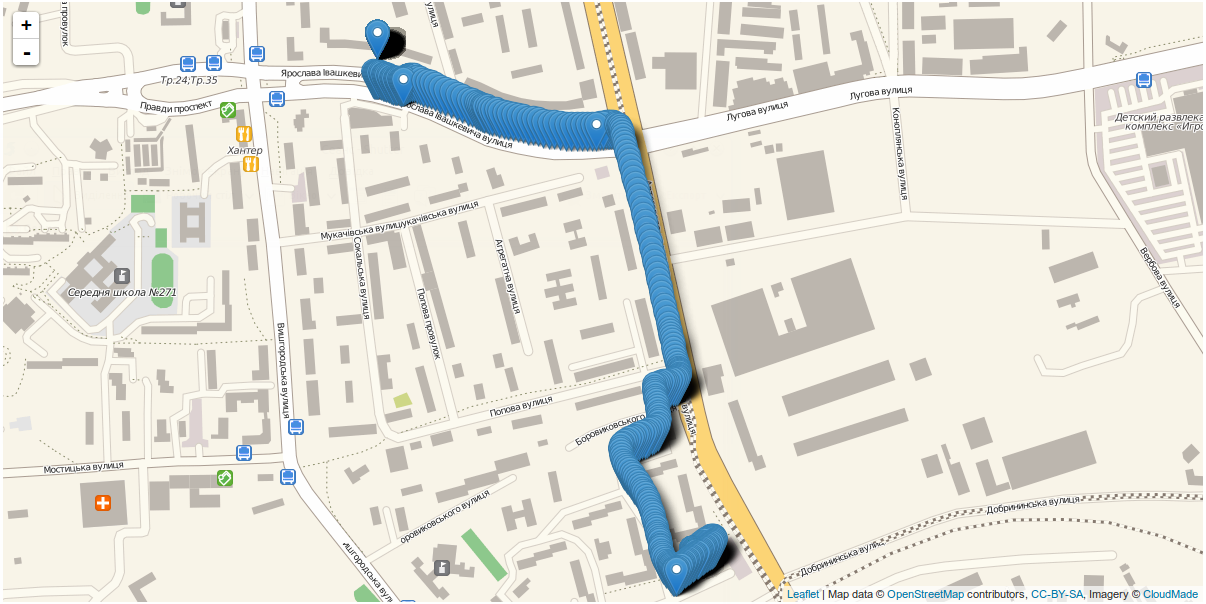
\includegraphics[scale=0.34]{images/leaflet_renderer.png}
    
    \newpage
    	
    \subsection{Відтворення шляху у вигляді двовимірного кістяка}
    
    Однією з перших поставлених цілей реалізації рендерера стояла реалізація алгоритму побудови двовимірного зображення пройденого маршруту, або ж його кістяка. 
    
    \textit{Кістяк маршруту} - це набір опорних точок чи ліній, на основі яких згодом будується пласка або тривимірна поверхня.
    
    Побудувавши плаский кістяк шляху у тривимірному просторі, можна вдосконалити його, піднявши ключові лінії на необхідну висоту та з’єднавши їх між собою поверхнями.
    
    З цією метою було сповна використано можливості графічного модуля бібліотеки \textbf{SFML}.
    
    Нижче наведено результати роботи першої та вдосконаленої версії алгоритмів.
    
    \vspace{3em}
    
    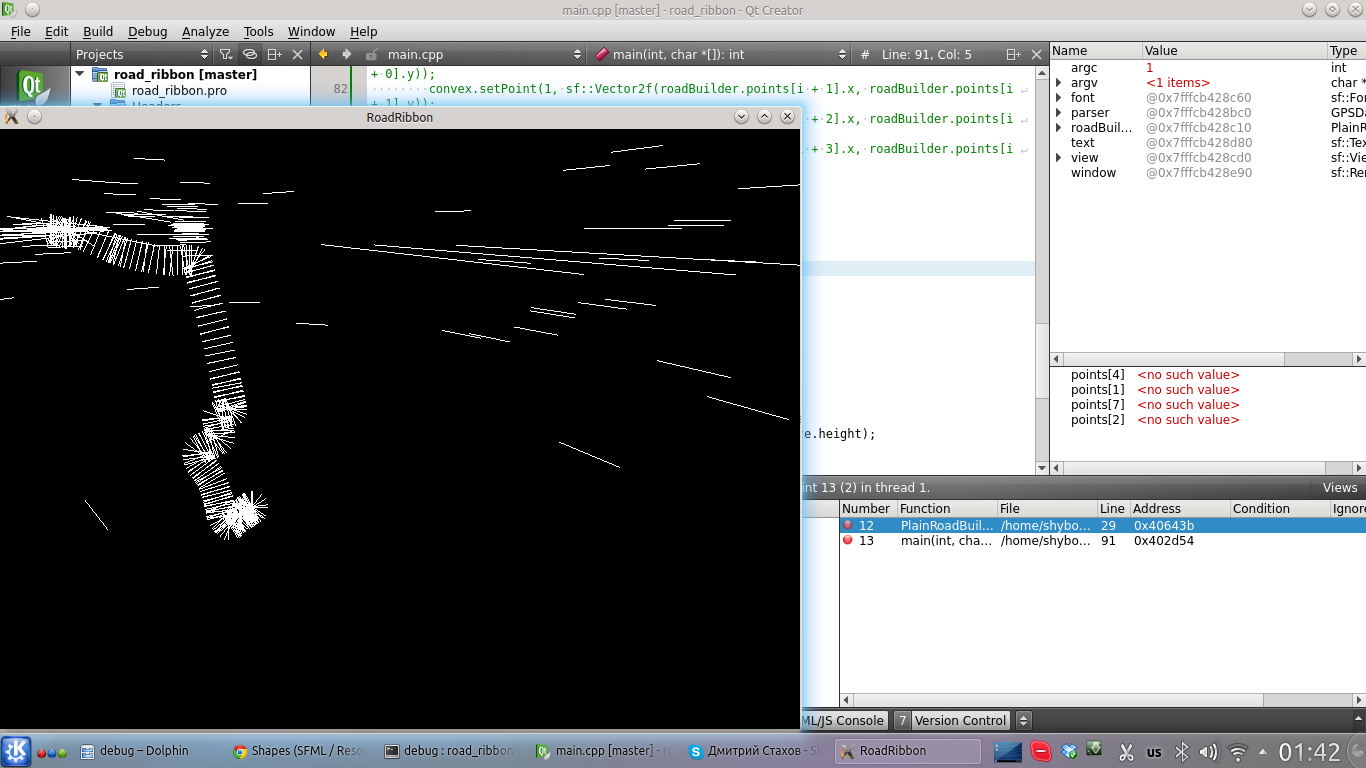
\includegraphics[scale=0.34]{images/road2d_1.png}
    
    \vspace{3em}
    
    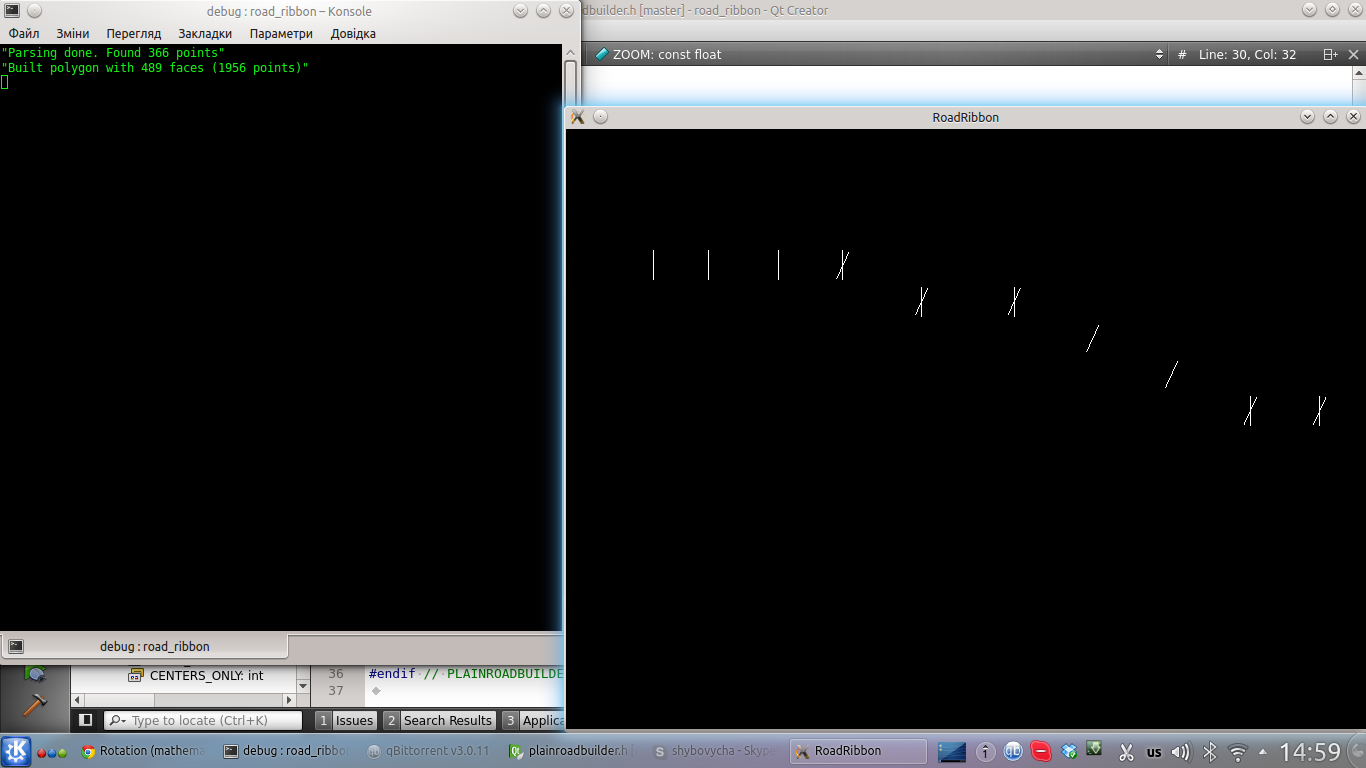
\includegraphics[scale=0.34]{images/road2d_2.png}
    
    \subsection{Побудова тривимірної поверхні}
    
    Для побудови тривимірної поверхні треку використовується один з двох підходів:
    
    \begin{enumerate}
    	\item \textbf{обробка даних гіродатчиків} - якщо інша опція недоступна
    	\item \textbf{обробка даних GPS} - використовуються зчитані дані про висоту над рівнем моря
    \end{enumerate}
    
    Якщо GPS-приймач на пристрої має змогу отримувати дані про висоту над рівнем моря в поточній позиції, ці дані будуть використані для побудови тривимірної поверхні треку. Так як дані цього типу не потребують додаткової обробки, даний метод найбільш приорітетний.
    
    Якщо ж GPS-приймач не надає можливості використовувати дані про висоту над рівнем моря, тоді мобільний агент перевіряє, чи доступний для використання так званий \textbf{G-серсор}. Якщо це вірно, то використовуються дані про поточний нахил GPS-приймача або смартфону та відстань до попереднього розташування (з використанням формули \textit{Great Circle Distance}) для отримання значення висоти, використовуючи властивості тригонометричних функцій.
    
    \subsection{Зміна перспективи огляду поверхні у просторі}
    
    Оскільки тривимірна поверхня треку в чистому вигляді (без фонових декорацій накшталт небесної сфери, ландшафту, предметів та будівель оточення, тощо) не дуже зручна для використання, було створено примітивний вказівник напрямків основних векторів тривимірного простору та додано орбітальну камеру, котра обертається довкола цього вказівника.
    
    Для зручного перегляду тривимірної поверхні дороги, камеру можна пересувати у восьми напрямках - вперед/назад, вгору/вниз та ліворуч/праворуч. Всі переміщення здійснюються відносно поточного розташування центру обертання камери - вказівника напрямних векторів простору.
    
    Обертання камери довкола центру обертання реалізовано за допомогою алгоритму множення кватерніонів.
    
    У поточній програмній реалізації рендерера це виглядає ось так:
    
    \vspace{3em}
    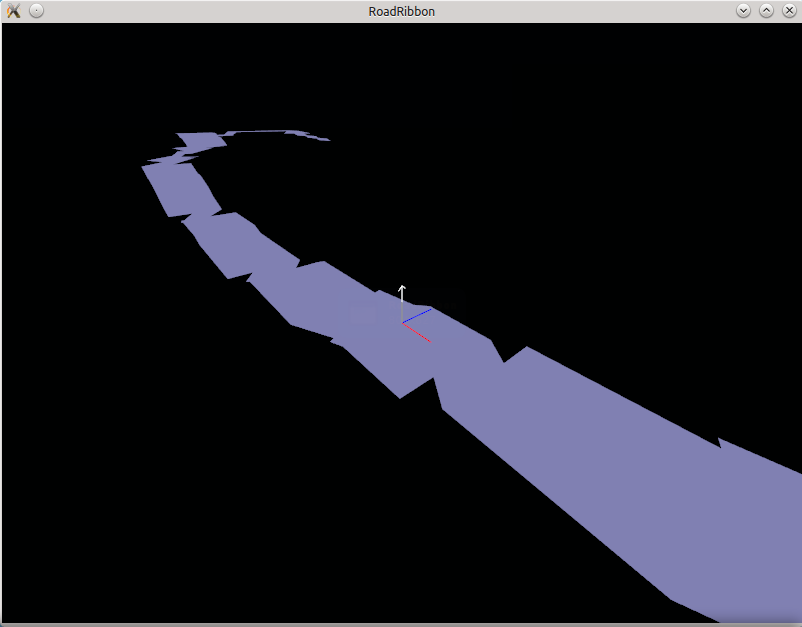
\includegraphics[scale=0.5]{images/camera1.png}
    
\newpage \section{Проектування системи}

    \subsection{Вибір інструментальних засобів}

        В якості мови програмування для створення мобільного агенту було обрано Java, так як

        \begin{itemize}
            \item мова містить лише необхідні та достатні для розробки конструкції
            \item мова компільована
            \item код мовою Java для розв’язку конкретно даної задачі виходить лаконічним та гнучким
            \item має чудову підтримку спільноти та гарну документацію - швидке вирішення більшості проблем за їх вникнення
            \item низький поріг входження - швидкий старт роботи з мовою програмування
            \item велика кількість готових рішень, написаного коду та бібліотек
        \end{itemize}
        
        Для створення рендерера було обрано мову програмування C++ за необхідності роботи з великими обсягами даних та тривимірним малюванням. 
        
        Для спрощення роботи було використано бібліотеки платформи Qt. Це дозволило спростити роботу з рядками, регулярними виразами та деякими контейнерними структурами даних.
        
        В якості бібліотеки для побудови та відображення двовимірної та тривимірної поверхні дороги було обрано OpenGL. Ця графічна система дозволяє просто та водночас ефективно працювати з двовимірними та тривимірними зображеннями та об’єктами. Поріг входження в цю систему значно нижчий за, скажімо, DirectX. А той факт, що система платформонезалежна дає змогу реалізувати рендерер для різних користувачів.
        
        З іншого ж боку, існуючі графічні чи ігрові двигунці та бібліотеки мають значно простіший інтерфейс для реалізації тих чи інших задач. Усі вони являють собою вищий рівень абстракції, ніж OpenGL чи DirectX. Але усі вони значно "важчі" для рішення задач подібного об’єму.
        
        Для створення контексту роботи OpenGL, обробки подій введення, створення та обробки зображень було використано бібліотеку SFML. Функціональні можливості цієї бібліотеки значно ширші за SDL, GLUT та інші, а програмний інтерфейс - простіший.

    \subsection{Загальна схема роботи системи}
    
    Всю схему роботи системи можна поділити на два етапи:
    
    \begin{enumerate}
    	\item \textbf{отримання даних про трек}
    	\item \textbf{візуалізація отриманих даних}
    \end{enumerate}
    
    Отримання даних - це процес подолання певного маршруту, під час якого у пам’яті смартфону відкладаються дані про поточне розташування мобільного агента.
    
    Під час подолання шляху мобільний агент постійно працює в режимі отримання геопозиційних даних від супутників мережі GPS. Тому цей процес є доволі енерго- та ресурсо-ємним для такого не надто потужного пристрою, як смартфон.
    
    Візуалізація даних відбувається на комп’ютері користувача. Уся обробка даних логічно розбита на кілька етапів:
    
    \begin{enumerate}
    	\item \textbf{дешифрація даних, отриманих від мобільних агентів}
    	\item \textbf{підготовка вершинних та індексних даних поверхні}
    	\item \textbf{відображення підготовлених даних у вигляді тривимірної поверхні}
    \end{enumerate}
    
    Дешифрація та підготовка даних до рендерингу - найбільш ресурсоємні процеси. Для дешифрації використовуються регулярні вирази, а для підготовки вершинних даних - повний перебір з використанням деякого математичного апарату. Обидва процеси виконують повний перебір усіх даних, що надійшли від мобільних агентів. Тому це найбільш тривалі у часі задачі.
    
    Відображення підготованих даних навантажує лише графічний процесор комп’ютера користувача. Для оптимізації цієї ділянки проекту було використано \textbf{VBO} - вершинні буфери.

	Нижче наведено діаграму загальної схеми роботи:
	
	\vspace{3em}
	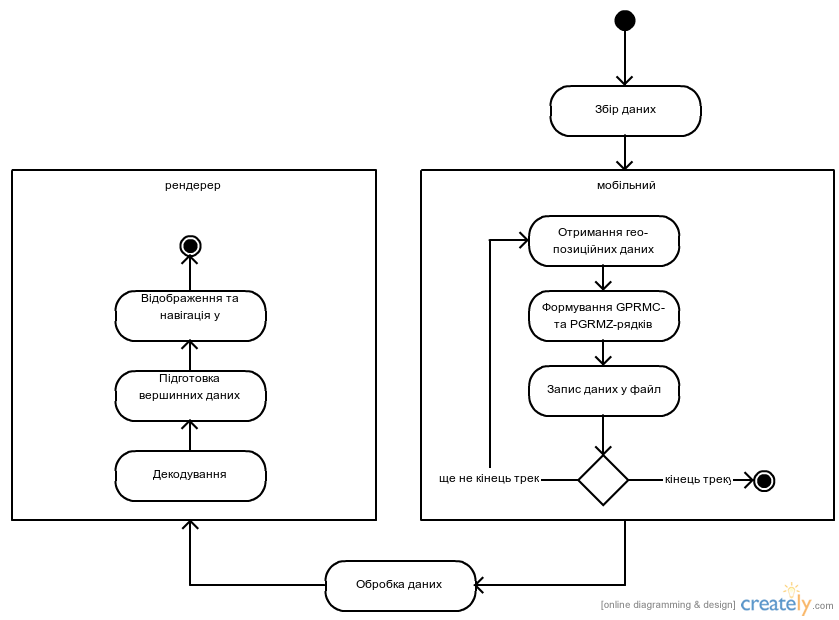
\includegraphics[scale=0.5]{images/general_workflow.png}

	\subsection{Архітектура мобільного агента}
	
	Мобільний агент складається з єдиного класу - \textit{MainActivity}. В цьому класі описано логіку завантаження мобільного додатку та основного циклу роботи додатку.
	
	При завантаженні, програма намагається приєднатись до супутників системи GPS та отримати геопозиційні дані. Як тільки їй це вдається, програма переходить в основний режим роботи - постійно зчитує та записує до файлу дані про положення мобільного агенту.
	
	Програма оновлює дані про гео-положення щосекунди. І щосекунди формує з отриманих даних два рядки - \textbf{рядок, що містить широту та довготу} та \textbf{рядок, що містить інформацію про рівень над рівнем моря}. Щоразу, коли рядки сформовано, програма додає їх до файлу на SD-карті пристрою.
	
	\textit{Оновлення файлу} (виконується приблизно щосекунди) - це набір операцій відкриття, запису та закриття файлу з даними. Виконання цих операцій щосекунди пов’язане з можливою помилкою, за якої дескриптор файлу даних залишиться у відкритому стані, якщо програма випадково завершиться. Тому, з метою збереження отриманих даних, відкриття та закриття файлу "обгортають" отримання та обробку даних.
	
	\vspace{2em}
	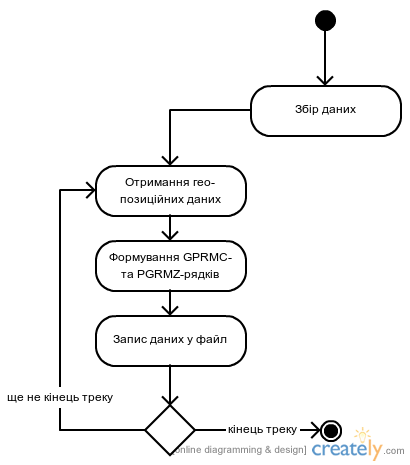
\includegraphics[scale=0.5]{images/mobile_agent_workflow.png}
        
    \subsection{Алгоритм отримання та збереження гео-даних}
    
    Отримавши дані від GPS-приймача, мобільний агент одразу ж формує з них два рядки:
    
    \begin{enumerate}
    	\item \textbf{рядок GPRMC} - дані про широту та довготу
    	\item \textbf{рядок PGRMZ} - дані про висоту над рівнем моря
    \end{enumerate}
    
	Формується два рядки наступного вигляду:
	
	\begin{lstlisting}
	$GPRMC,113138.00,A,5026.59,N,3021.22,E,,,160114,,,A
	$PGRMZ,195,m,3
	\end{lstlisting}
    
    Збереження відбувається у файл, ім’я якого містить часовий штамп - дату та час початку збору даних мобільним агентом. Це дозволяє сортувати дані ще на етапі міграції даних з мобільного агента на комп’ютер користувача.
    
    Тут слід відмітити, що за стандартом NMEA-0183, широта та довгота записуються у форматі \textbf{DDMM.MM}, де \textbf{DD} - дві цифри градусної міри кута, а \textbf{MM.MM} - хвилини та кількість секунд у вигляді частини хвилини.
    
    Тобто, якщо широта гео-локації рівна $50^\circ 44' 15''$, то у форматі NMEA-0183 ця величина буде рівна $50^\circ; 44' + (\frac{15}{60})' = 50^\circ 44.25'$ і записана як як $5044.25$
    
    Структура мобільного агента мінімальна для зниження ресурсовитрат смартфону. Нижче наведена діаграма класів мобільного агента.
    
    \vspace{3em}
    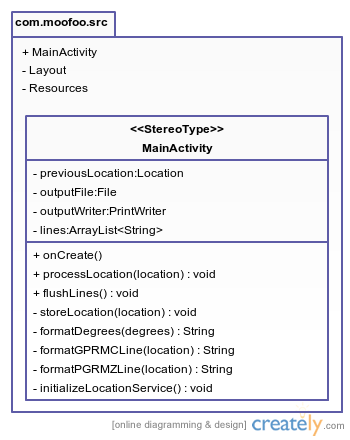
\includegraphics[scale=0.75]{images/mobile_agent_classes.png}

    \subsection{Архітектура рендерера}
    
    Рендерер - найбільш ресурсоємна частина системи. Вона складається з кількох класів, кожен з яких несе відповідальну роль в побудові результуючого зображення.
    
    Нижче наведена діаграма діяльності та діаграма класів рендерера:
    
    \vspace{3em}
	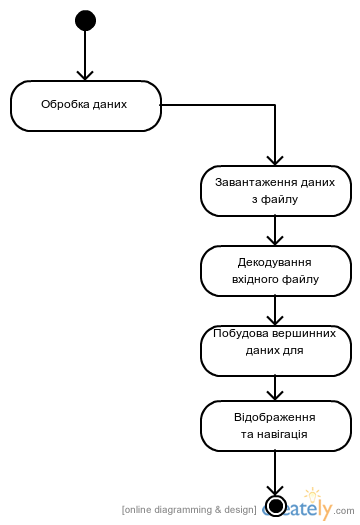
\includegraphics[scale=0.5]{images/renderer_workflow.png}
	
	\newpage
	\begin{landscape}
		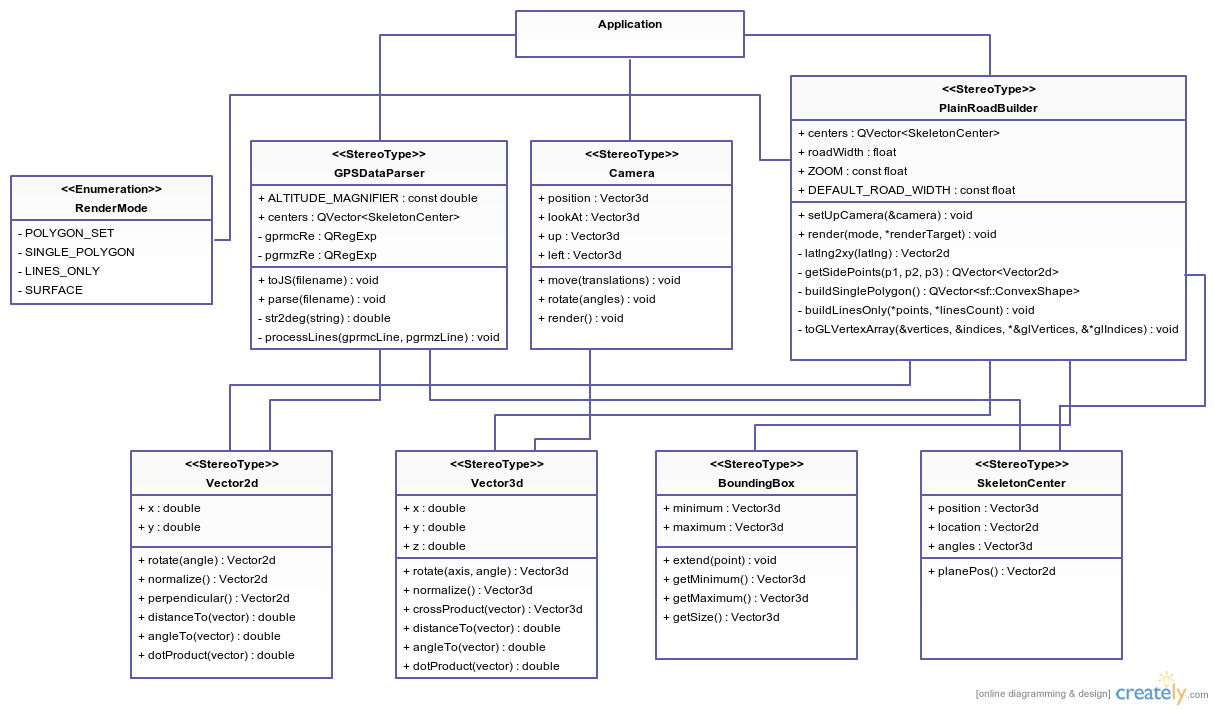
\includegraphics[scale=0.5]{images/renderer_classes.png}
	\end{landscape}

	\subsection{Алгоритм завантаження даних}
	
	Формат даних мобільного агента вимагає, аби за кожним рядком, що містить дані про розташування йшов рядок, що містить дані про висоту над рівнем моря у цьому розташуванні. Тому для дешифрування файлу даних створено два регулярних вирази:
	
	\begin{enumerate}
		\item \textbf{gprmcRe} - регулярний вираз для розбору рядка з розташуванням
		\item \textbf{pgrmzRe} - регулярний вираз для розбору рядка з інформацією про висоту над рівнем моря
	\end{enumerate}
	
	З файлу даних в циклі зчитується по два рядки, після чого кожен з них перевіряється на відповідність своєму регулярному виразу. Якщо бодай один з рядків не відповідає шаблону - поточна ітерація пропускається та виводиться відповідне повідомлення про помилку.
	
	Після порівняння з шаблоном, зчитані два рядки розбиваються на відповідні груповані частини тексту, вказані у регулярних виразах. Кожна зі знайдених частин рядка перетворюється у відповідності до інформації, що вона несе в собі. Так, виділяються \textbf{широта}, \textbf{довгота} (перетворені у десятковий формат) та \textbf{висота над рівнем моря}. Усі ці дані заповнюють об’єкт класу \textbf{SkeletonCenter} (\textit{центр кістяка}).
	
	Отриманий набір центральних вузлів передається на метод побудови двовимірного кістяка дороги, або ж тривимірної поверхні треку - в залежності від режиму побудови.
	
	\subsection{Алгоритм побудови двовимірного кістяка дороги}
	
		Отримана послідовність центральних вузлів кістяка очищується від дубльованих центрів. Тобто, з неї викидаються усі центральні вузли, відстань між якими (за формулою відстані між двома векторами \textbf{на площині}, що дає значно більш точні результати, аніж \textit{Great Circle Distance}) менша за порогове значення (\textit{0.01 м}).
		
		Після цього, кожному центральному вузлові кістяка асоціюється пара \textit{бокових} вершин, які утворюють відрізок. Умовою побудови цього відрізка є перпендикулярність лінії, що з’єднує поточний центровий вузел кістяка дороги з наступним та попереднім центровими вузлами. 
		
		Але оскільки одна лінія не може бути перпендикулярна двом іншим, не паралельним між собою, лініям, то в якості результуючого ребра кістяка обирається такий відрізок, який лежить на бісектрисі кута між перпендикулярами до відрізків, що з’єднують два несуміжні центрові вузли треку.
		
		Якщо, наприклад, потрібно утворити ребро кістяка треку для центрального вузла B (\textit{див. мал.}), тоді потрібно аналізувати попередній до нього у списку центрових вузлів вузол (A) та наступний за ним вузол у списку центрових вузлів (C). Знаходяться два перпендикуляри до прямих, що з’єднують пари центральних вузлів: $c \perp AB$ та $d \perp BC$. Визначається кут між цими перпендикулярами $\alpha = \measuredangle(c, d)$. Визначається градусна міра половини цього кута, $\beta = \frac{\alpha}{2}$ та з точки $B$ відкладається вектор $\overline{a}$, довжина якого рівна половині ширини майбутньої дороги, повернутий на кут $\beta$: $\overline{BF} = \overline{AB} + \overline{a} \circlearrowright \beta$. Аналогічна операція проводиться і для вектора $\overline{BG}$. Таким чином отримується пара вершин $F$ та $G$, які і утворюють ребро для центрового вузла $B$.
		
		\vspace{3em}
		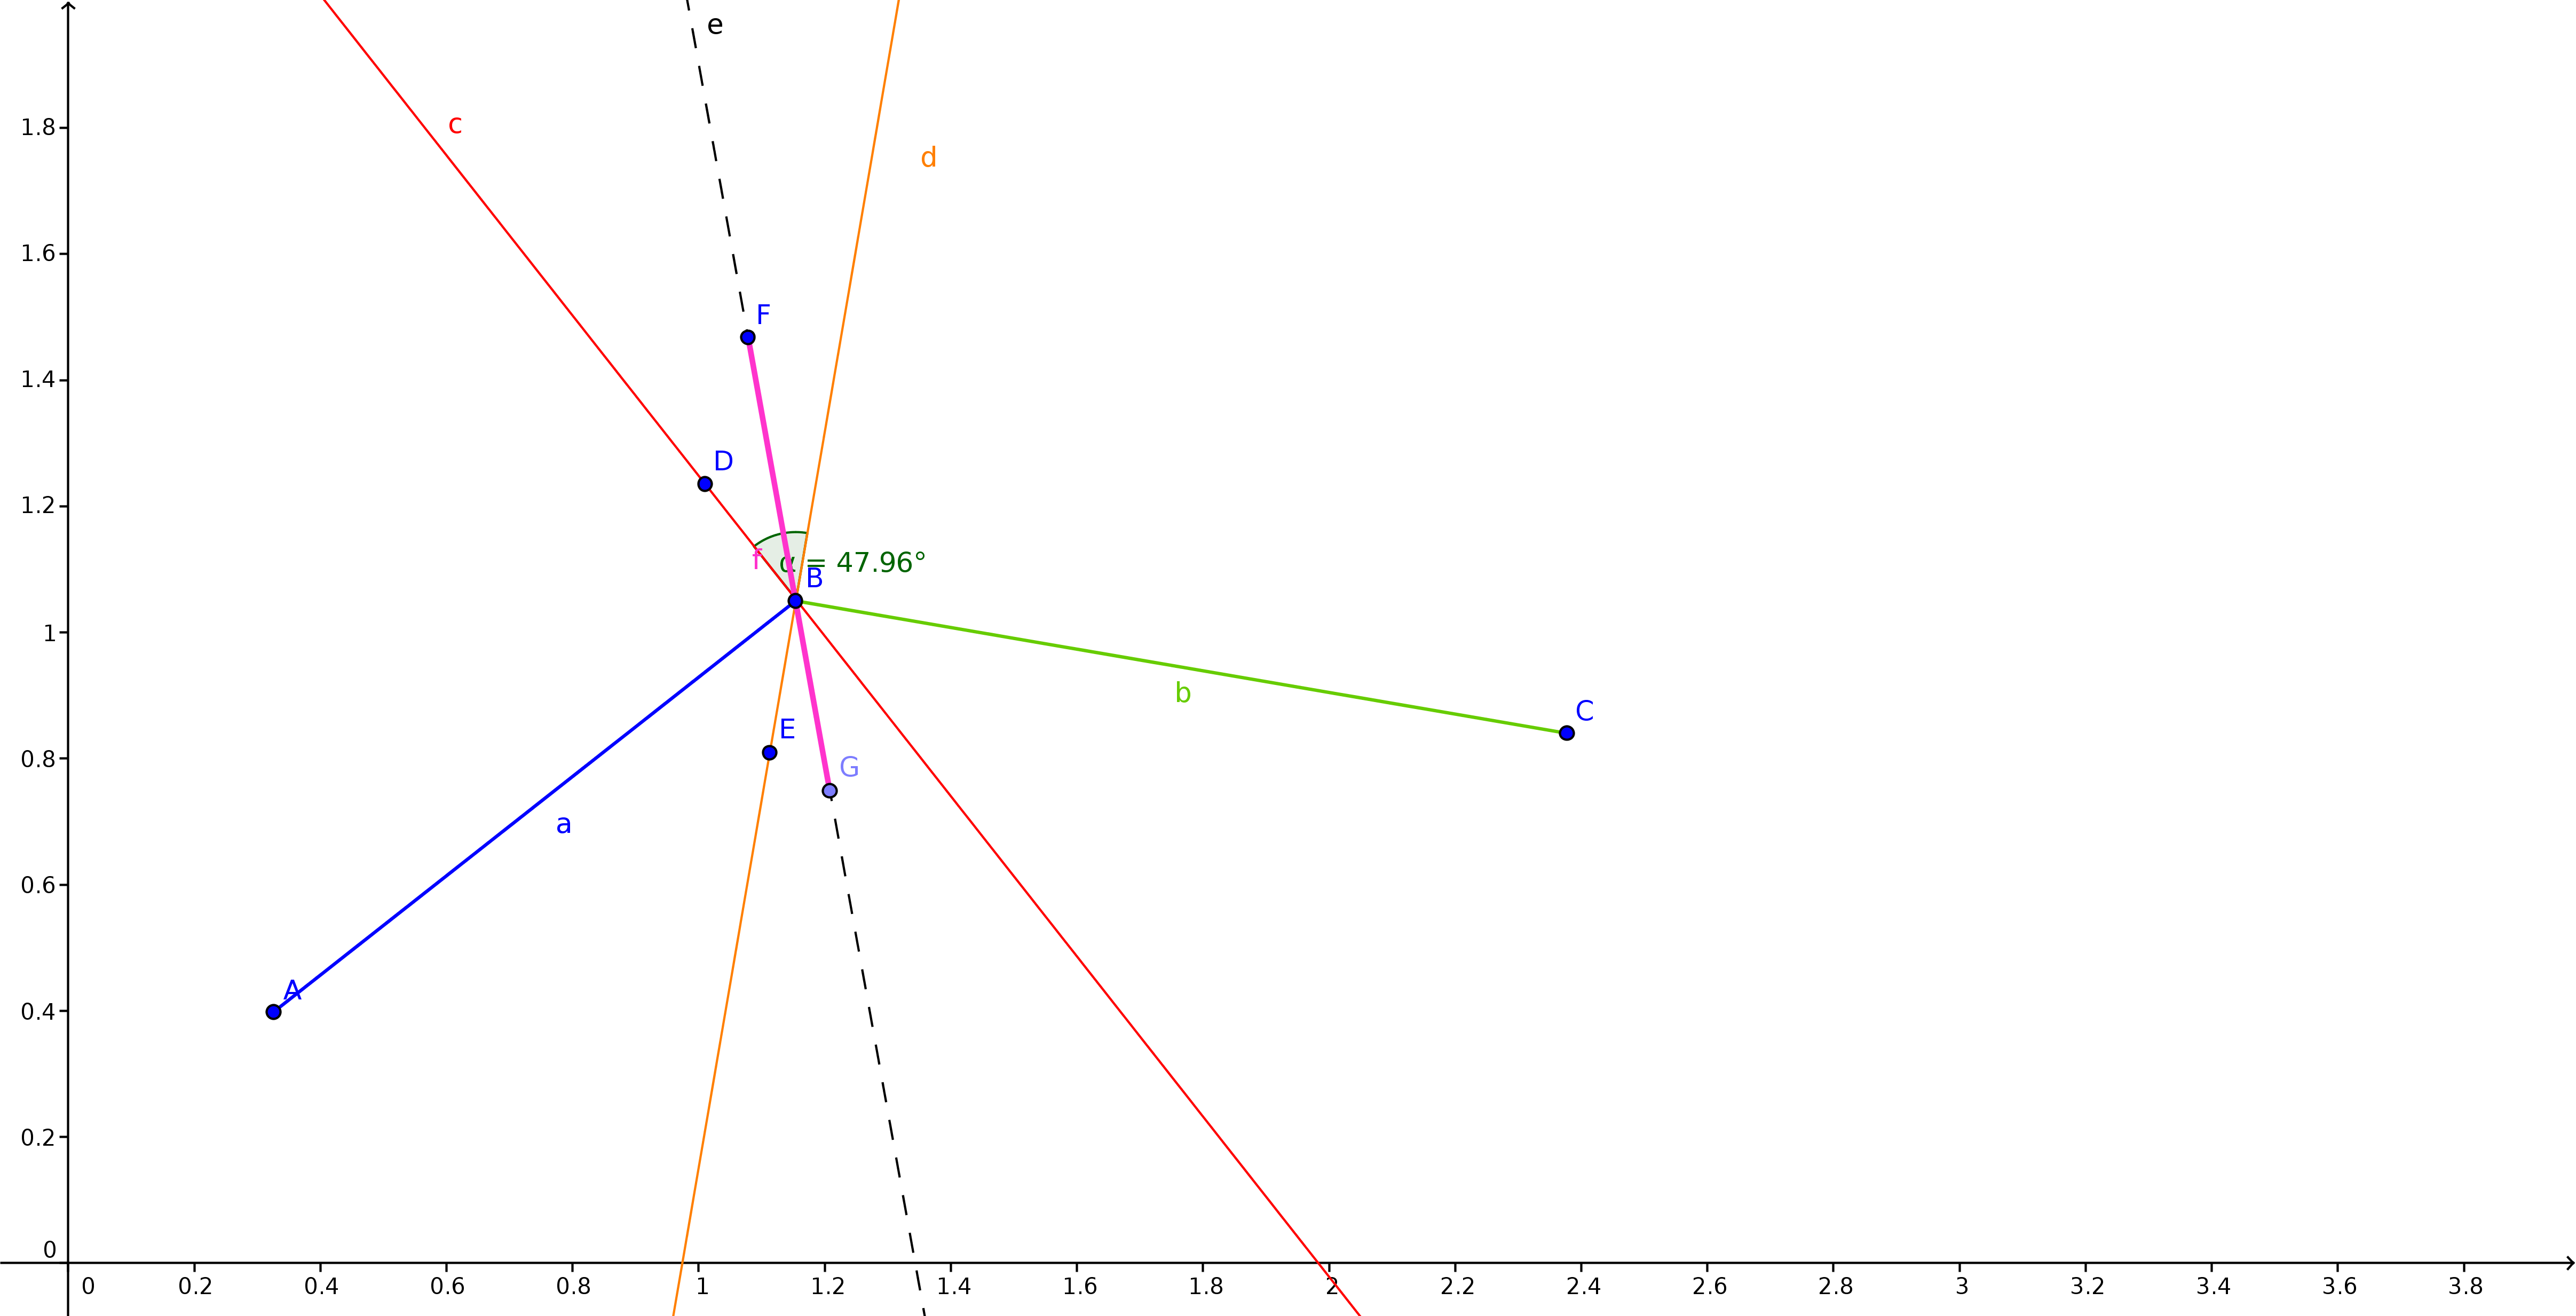
\includegraphics[scale=0.65]{images/perpendicular_1_1.png}
	
	\subsection{Алгоритм побудови тривимірної поверхні дороги}
	
		Отримана послідовність центральних вузлів кістяка очищується від дубльованих центрів. Тобто, з неї викидаються усі центральні вузли, відстань між якими (за формулою відстані між двома векторами \textbf{у просторі}, що дає значно більш точні результати, аніж \textit{Great Circle Distance}) менша за порогове значення (\textit{0.01 м}).
		
		Всі операції в точності повторюють алгоритм побудови двовимірного кістяка лише з двома поправками:
		
		\begin{enumerate}
			\item \textbf{центрові вузли піднімаються на висоту $h$} - для двовимірного кістяка висота не грала ролі, в той час як для тривимірної поверхні даний критерій є ключовим
			\item \textbf{вершини додаються до списку у заданому порядку} - для подальшого відображення поверхні засобами OpenGL необхідно надати вершини, упорядковані та груповані у чотирикутні сети - впорядковані підмножини з чотирьох елементів, котрі утворять черговий сегмент майбутньої поверхні
		\end{enumerate}
		
		В результаті отримується список, у котрому кожному центровому вузлу відповідає чотири впорядковані вершини - дві з яких утворюють ребро кістяка дороги для попереднього центрового вузла, а дві - для поточного.
	
	\subsection{Навігація у просторі рендерера}
	
		Навігація у просторі створена для більш зручного перегляду отриманої тривимірної поверхні дороги. З цією метою і створений клас \textbf{Camera}. Він цілком відповідає за задання матриці перегляду моделі. Єдина частина рендерера, котра не належить цьому класу але відповідає за зміну перспективи знаходиться в головній функції програми та відповідає за обробку натиснень користувачем клавіш на клавіатурі з метою керування камерою.
		
		Камера являє собою уявну точку (точка огляду, \textbf{eyePos}), з якої ведеться огляд іншої точки (\textbf{lookAt}). Камера обертається довкола точки обертання (\textbf{lookAt}), постійно знаходячись на однаковій відстані від неї. Такий спосіб навігації у віртуальному просторі видався автору найбільш зручним для користувача.
		
		Точку обертання можна переміщувати вздовж треку. Це дає змогу переглянути всю поверхню дороги з усіх боків (враховуючи обертання камери довкола точки огляду). Разом з переміщенням точки обертання, на ідентичну відстань переміщується і точка, з якої якої ведеться спостереження, точка огляду. Це створює приємний ефект переміщення камери.
		
		Точка огляду обертається довкола точки обертання використовуючи таку математичну структуру даних як \textbf{кватерніон}; зокрема - властивість множення кватерніонів.
		
		\vspace{3em}
		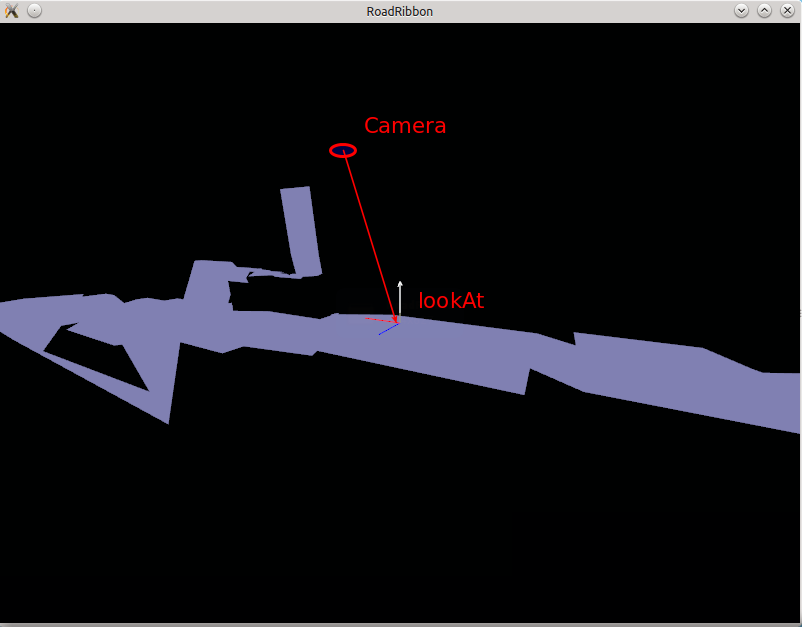
\includegraphics[scale=0.5]{images/camera2.png}
       
\newpage \section{Функціональний опис архітектури системи}

    \subsection{Модуль мобільного агента}

        \subsubsection{Призначення та короткий опис модуля}

            Даний модуль описує базові математичні структури, що використовуються в програмі в подальшому, та математичні операції над цими структурами. Даний модуль містить базові класи, котрі наслідуються в усіх наступних модулях.

        \subsubsection{Клас MainActivity}
        
        	\textbf{Обробник події створення програми}
        	
        	При створенні програми викликається подія \textit{onCreate}. Її перехоплює та оброблює відповідний метод класу \textbf{MainActivity}. Під час ініціалізації створюється інтерфейс програми та ініціюється процес отримання даних з GPS-приймача. В цей же момент описуються обробники події отримання даних з GPS-приймача.
        	
        	\begin{lstlisting}[language=Java]
@Override
protected void onCreate(Bundle savedInstanceState) {
    super.onCreate(savedInstanceState);

    setContentView(R.layout.activity_main);

    if (savedInstanceState == null) {
        getSupportFragmentManager().beginTransaction()
                .add(R.id.container, 
                	new PlaceholderFragment())
                .commit();
    }

    initializeLocationService();
}
        	\end{lstlisting}
        	
        	\textbf{Обробник події отримання гео-даних}
        	
        	Ця ділянка мобільного агенту перехоплює подію зміни позиції (або ж отримання оновлених даних про позицію).
        	
        	Стиль програмування вимагає максимального розбиття цілісного методу на мінімальні складові з метою подальшої модифікації окремих шматочків системи, а не великого цілого. Тому обробник події зміни позиції просто передає дані про нове положення методу обробки позиції.
        	
\begin{lstlisting}[language=Java]
public void onLocationChanged(Location location) {
	MainActivity.this.processLocation(location);
}
\end{lstlisting}

			Той, в свою чергу, передає керування методу збереження положення \textbf{тоді і лише тоді}, коли нове положення відрізняється від останнього збереженого.
			
\begin{lstlisting}[language=Java]
protected void processLocation(Location location) {
    if ((this.previousLocation != null && 
    	location.distanceTo(this.previousLocation) > 
    		Math.pow(1.0, -3.0)
    	) || (this.previousLocation == null)
   	) {
        this.storeLocation(location);
    }

    this.previousLocation = location;
}
\end{lstlisting}

			Збереження положення поділене на два етапи:
			
			\begin{enumerate}
				\item \textbf{формування двох текстових рядків}, які містять інформацію про положення та висоту над рівнем моря в цій гео-позиції; якщо обидва рядки корректно сформовані - вони додаються до черги на запис у файл
				\item \textbf{запис даних у файл} - відбувається виштовхування всіх накопичених рядків з черги у файл
			\end{enumerate}
			
\begin{lstlisting}[language=Java]
protected void storeLocation(Location location) {
    try {
        String gprmcLine = this.formatGPRMCLine(location);
        String pgrmzLine = this.formatPGRMZLine(location);

        this.lines.add(gprmcLine);
        this.lines.add(pgrmzLine);

        this.addTextMessage(gprmcLine);
        this.addTextMessage(pgrmzLine);

        this.flushLines();
    } catch (Exception e) {
        // ...

        return;
    }
}
\end{lstlisting}
        	
        	\textbf{Метод форматування рядків з даними}
        	
        	Рядки формуються за допомогою можливостей форматування рядків, дат та чисел Java.
        	
\begin{lstlisting}[language=Java]
protected String formatDegrees(double lat) {
    long D = Math.round(lat);
    double m = (lat - D) * 60.0;
    DecimalFormatSymbols otherSymbols = new 
    	DecimalFormatSymbols(Locale.UK);

    String res = String.format("%02d%s",
            D,
            new DecimalFormat("##.##", otherSymbols).format(m)
    );

    return res;
}

protected String formatGPRMCLine(Location location) {
    String lat = this.formatDegrees(location.getLatitude());
    String lng = this.formatDegrees(location.getLongitude());

    Calendar cal = Calendar.getInstance();
    String time = new SimpleDateFormat("HHmmss.00").format(
    	cal.getTime()
    );
    String date = new SimpleDateFormat("ddMMyy").format(
    	cal.getTime()
    );

    return String.format(
            "$GPRMC,%s,A,%s,N,%s,E,,,%s,,,A\r\n",
            time,
            lat,
            lng,
            date
    );
}

protected String formatPGRMZLine(Location location) {
    // $PGRMZ,93,m,3 - altitude
    long alt = Math.round(location.getAltitude());

    return String.format(
            "$PGRMZ,%02d,m,3\r\n",
            alt
    );
}
\end{lstlisting}
        	
        	\textbf{Метод запису даних у файл}
        	
        	Для запису у файл створюється об’єкт класу \textit{File} з іменем, що містить поточну дату та час. Якщо такий файл вже існує - дані будуть додані у кінець цього файлу. Файл створюється в кореневому каталозі SD-карти смартфону.
        	
        	Після відкриття відповідного файлу, дані з черги записуються у файл, а сама черга - очищається.
        	
\begin{lstlisting}[language=Java]
protected void flushLines() {
    try {
        if (this.outputFile == null) {
            Calendar cal = Calendar.getInstance();
            String filename = String.format(
            	"roadribbon_%s.txt",
                new SimpleDateFormat("ddMMyyyy_hhmmss").
                	format(cal.getTime())
            );

            File dir = new File(
            	Environment.getExternalStorageDirectory(), 
            	"/RoadRibbon"
            );
            dir.mkdirs();

            this.outputFile = new File(dir, filename);
        }

        FileOutputStream stream = new FileOutputStream(
        	this.outputFile, true
        );
        this.outputWriter = new PrintWriter(stream);

        for (String line : this.lines) {
            this.outputWriter.print(line);
        }

        this.outputWriter.close();

        this.lines.clear();
    } catch (Exception e) {
        // ...

        return;
    }
}
\end{lstlisting}
        
     \subsection{Модуль рендерера}
     
     	\subsubsection{Клас Vector2d}
     	
     		Даний клас описує вектор на площині та деякі операції над векторами на площині, як, наприклад, \textit{поворот}, \textit{визначення кута між двома векторами}, \textit{визначення вектору}, \textit{перпендикулярного до даного}, \textit{нормалізація вектора}, тощо.
     	
        	\textbf{Конструктор класу}

            \begin{lstlisting}[language=C++]
            Vector2d(_x = 0.0, _y = 0.0);
            \end{lstlisting}

            По замовчуванню всі координати вектора задані нульовими, тож можливий варіант виклику конструктора:

            \begin{lstlisting}
            new Vector2d(); 
            \end{lstlisting}     	
     	
	     	\textbf{Визначення вектора-перпендикуляра}
	     	
	     	Якщо дано вектор, $\overline{a} (x_1, y_1)$ тоді вектор $\overline{b} (x_2, y_2) \perp \overline{a}$ якщо $\overline{a} \cdot \overline{b} = 0$.
	     	
	     	Для того, щоб знайти координати перпендикулярного вектора необхідно розв’язати два рівняння:
	     	
	     	$$
	     		\overline{b}(x_2, y_2) \perp \overline{a}(x_1, y_1) \Rightarrow (x_1 \cdot x_2) + (y_1 \cdot y_2) = 0;
	     	$$
	     	
			Припустимо, що $x_2 = 1$. Тоді:
	     	
	     	$$
	     		x_1 + y_1 \cdot y_2 = 0 \Rightarrow y_2 = -\frac{x_1}{y_1}
	     	$$
	     	
	     	Так само знаходиться й $x_2$:
	     	
	     	$$
	     		y_2 = 1 \Rightarrow x_1 \cdot x_2 + y_1 = 0 \Rightarrow x_2 = -\frac{y_1}{x_1}
	     	$$
     	
    	\subsubsection{Клас Vector3d}

            Даний клас описує вектор у просторі та деякі операції над векторами.

            \textbf{Конструктор класу}

            \begin{lstlisting}[language=C++]
            Vector3d(_x = 0.0, _y = 0.0, _z = 0.0);
            \end{lstlisting}

            По замовчуванню всі координати вектора задані нульовими, тож можливий варіант виклику конструктора:

            \begin{lstlisting}
            new Vector3d(); 
            \end{lstlisting}

            \textbf{Операції над векторами}

            Даний клас описує більшість необхідних операцій над векторами, як-то: множення та ділення на скаляр та на вектор, додавання та віднімання. Також описані додаткові мктоди: визначення модуля вектора (\textit{\textbf{length}}), порівняння рівності та нерівності векторів (\textit{\textbf{==}}, \textit{\textbf{!=}}), визначення кута між двома векторами (\textit{\textbf{angle\_to(vector)}}), поворот навколо заданої осі на заданий кут (\textit{\textbf{rotate(angle, axis)}}).

            Визначення кута між двома векторами реалізовано за допомогою формули скалярного добутку векторів:

            $$ \phi = \arccos \frac{\vec{a}\vec{b}}{\abs{\vec{a}}\abs{\vec{b}}} $$

            Поворот вектора навколо заданої осі на заданий кут реалізовано за допомогою розгорнутої форми множення кватерніонів:


            Нехай $\vec{u}$ - вектор-вісь, навколо якої обертатимемо вектор; $\vec{v}$ - вектор, котрий обертатимемо, а $\alpha$ - кут, на який обертатимемо $\vec{v}$ навколо вісі $\vec{u}$.

            Якщо кватерніон $ q = \cos \frac{\alpha}{2} + \vec{u} \sin \frac{\alpha}{2} $, то

            $$ \vec{v'} = q \vec{v} q^{-1} = \left( \cos \frac{\alpha}{2} + \vec{u} \sin \frac{\alpha}{2} \right) \, \vec{v} \, \left( \cos \frac{\alpha}{2} - \vec{u} \sin \frac{\alpha}{2} \right) $$

            або

            \begin{displaymath}
                \begin{array}{lll}
                    \vec{v'} &=& \vec{v} \cos^2 \frac{\alpha}{2} + (\vec{u}\vec{v} - \vec{v}\vec{u}) \sin \frac{\alpha}{2} \cos \frac{\alpha}{2} - \vec{u}\vec{v}\vec{u} \sin^2 \frac{\alpha}{2} \\
                    &=& \vec{v} \cos^2 \frac{\alpha}{2} + 2 (\vec{u} \times \vec{v}) \sin \frac{\alpha}{2} \cos \frac{\alpha}{2} - (\vec{v} (\vec{u} \cdot \vec{u}) - 2 \vec{u} (\vec{u} \cdot \vec{v})) \sin^2 \frac{\alpha}{2} \\
                    &=& \vec{v} (\cos^2 \frac{\alpha}{2} - \sin^2 \frac{\alpha}{2}) + (\vec{u} \times \vec{v}) (2 \sin \frac{\alpha}{2} \cos \frac{\alpha}{2}) + \vec{u} (\vec{u} \cdot \vec{v}) (2 \sin^2 \frac{\alpha}{2}) \\
                    &=& \vec{v} \cos \alpha + (\vec{u} \times \vec{v}) \sin \alpha + \vec{u} (\vec{u} \cdot \vec{v}) (1 - \cos \alpha) \\
                    &=& (\vec{v} - \vec{u} (\vec{u} \cdot \vec{v})) \cos \alpha + (\vec{u} \times \vec{v}) \sin \alpha + \vec{u} (\vec{u} \cdot \vec{v})
                \end{array}
            \end{displaymath}

        \subsubsection{Клас GPSDataParser}
        
        \textbf{Короткий опис класу}
        
        Даний клас призначений для зчитування та дешифрування даних, отриманих в результаті роботи мобільних агентів під час подолання ними певних маршрутів.
        
        Клас дає змогу перетворити файл з даними або у скрипт мовою програмування \textbf{JavaScript}, який можна використати для перегляду пройденого мобільним агентом маршруту на мапі (за допомогою наявної HTML-сторінки в директорії \textbf{test}), або у набір центрових вузлів маршруту.
        
        \textbf{Конструктор}
        
        В конструкторі об’єкту класу \textbf{GPSDataParser} створюється два регулярних вирази - по одному на кожен з рядків, які "розуміє" рендерер:
        
\begin{small}
\begin{lstlisting}[language=C++]
void GPSDataParser::init()
{
gprmcRe = QRegExp("\\$GPRMC,((\\d\\d)(\\d\\d)(\\d+\\.\\d+)),([A-Z])...");

pgrmzRe = QRegExp("\\$PGRMZ,(\\d+),(m|f),(\\d+)");

centers.clear();
}
\end{lstlisting}
\end{small}
        
        \textbf{Конвертація у JS-файл}
        
        При конвертації у JavaScript-файл (з метою подальшого використання у HTML-сторінці, на якій відображається мапа з пройденим мобільним агентом маршрутом) створюється файл, котрий задає об’єкту \textbf{window} поле \textbf{waypoints} - масив пар координат, що відповідають конкретному центровому вузлу кістяка маршруту.

\begin{small}        
\begin{lstlisting}[language=C++]
void GPSDataParser::toJS(QString filename)
{
    if (centers.size() < 1)
    {
        return;
    }

    QFile f(filename);

    f.open(QIODevice::WriteOnly | QIODevice::Text);

    QTextStream out(&f);

    out << "window.waypoints = [\n";

    for (long long i = 0; i < centers.size(); i++)
    {
        QString line = QString("[ %1, %2 ]").
        	arg(centers[i].location.x).
        	arg(centers[i].location.y);

        out << line;

        if (i < centers.size() - 1)
        {
            out << ",";
        }

        out << "\n";
    }

    out << "];";

    f.close();
}
\end{lstlisting}
\end{small}

		\textbf{Методи обробки рядку гео-позиції}
		
		Методи використовують створені у конструкторі регулярні вирази та зчитані з файлу даних рядки.
		
\begin{small}
\begin{lstlisting}[language=C++]
double GPSDataParser::str2deg(QString str)
{
    QRegExp lat_re("(\\d\\d)(\\d\\d\\.\\d+)"),
            lng_re("(\\d\\d\\d)(\\d\\d\\.\\d+)");

    double degrees = 0.0, minutes_part = 0.0;

    if (lat_re.indexIn(str) != -1)
    {
        degrees = lat_re.cap(1).toDouble();
        minutes_part = lat_re.cap(2).toDouble();

        return degrees + (minutes_part / 60.0);
    } else if (lng_re.indexIn(str) != -1)
    {
        degrees = lng_re.cap(1).toDouble();
        minutes_part = lng_re.cap(2).toDouble();

        return degrees + (minutes_part / 60.0);
    } else
    {
        return 0.0;
    }
}

void GPSDataParser::processLines(QString gprmcLine, QString pgrmzLine)
{
    if (gprmcRe.indexIn(gprmcLine) < 0)
    {
        return;
    }

    if (pgrmzRe.indexIn(pgrmzLine) < 0)
    {
        return;
    }

    Vector2d location = processGPRMCLine(gprmcLine);
    double alt = processPGRMZLine(pgrmzLine) * ALTITUDE_MAGNIFIER;
    Vector3d position = Vector3d(location.x, alt, location.y);

    // TODO: refactor
    SkeletonCenter center(location, position, Vector3d(0, 0, 0));

    centers.push_back(center);
}

Vector2d GPSDataParser::processGPRMCLine(QString line)
{
    gprmcRe.indexIn(line);

    double lat = str2deg(gprmcRe.cap(6)),
           lng = str2deg(gprmcRe.cap(10));

    return Vector2d(lat, lng);
}

double GPSDataParser::processPGRMZLine(QString line)
{
    pgrmzRe.indexIn(line);

    return pgrmzRe.cap(1).toDouble();
}
\end{lstlisting}
\end{small}

        \subsubsection{Клас PlainRoadBuilder}
        
        \textbf{Которкий опис класу}
        
        Даний клас використовується для приведення послідовності центрових вузлів кістяка маршруту до вигляду, зручного для використання бібліотекою OpenGL.
        
        \textbf{Конструктор класу}
        
        В конструкторі послідовність центральних вузлів фільтрується з метою прибрати ідентичні центри, а також кожному центру задається позиція в координатах простору.
        
\begin{small}
\begin{lstlisting}[language=C++]
PlainRoadBuilder::PlainRoadBuilder(QVector<SkeletonCenter> _centers, 
	float roadWidth
)
{
    if (_centers.size() < 3)
    {
        return;
    }

    Vector2d origin = this->latlng2xy(_centers[0].location);

    for (int i = 1; i < _centers.size(); i++)
    {
        while ((i < _centers.size() - 1) && 
        	(_centers[i + 1].location == _centers[i].location)
        ) i++;

        SkeletonCenter center = _centers[i];

        Vector2d xy = this->latlng2xy(centers[i].location, 
        	origin
        );

        center.position = Vector3d(xy.x, 
        	centers[i].position.y * (ZOOM * 4), 
        	xy.y
       	);

        this->centers.push_back(center);
    }

    this->roadWidth = roadWidth;
}
\end{lstlisting}
\end{small}
        
        \textbf{Перетворення широти та довготи в координати у просторі}
        
        \textbf{Побудова вершинних даних}
        
        Для побудови вершинних даних використовуються дані про ребро, що асоційоване з попереднім до поточного оброблюваного центрового вузла дороги.
        
\begin{small}
\begin{lstlisting}[language=C++]
void PlainRoadBuilder::buildPolygonSet(
	QVector<Vector3d>* vertices, QVector<int>* indices
)
{
    for (int i = 1; i < this->centers.size() - 1; i++)
    {
        Vector2d A = this->centers[i - 1].planePos(),
                B = this->centers[i].planePos(),
                C = this->centers[i + 1].planePos(),
                BA = A - B;

        double angle = 0; // M_PI / 16.0;

        if (fabs((C - B).angleTo(A - B) - M_PI) < pow(10.0, -5.0))
        {
            angle = 0;
        }

        Vector2d a = BA.perpendicular().
        			normalize().
        			rotate(angle) * this->roadWidth,
                AL = A + a,
                AR = A - a;

        Vector3d AL3D = 
        	Vector3d(AL.x, this->centers[i].position.y, AL.y),
                AR3D = 
            Vector3d(AR.x, this->centers[i].position.y, AR.y);

        int index = vertices->size();

        if (i == 1)
        {
            vertices->push_back(AL3D);
            vertices->push_back(AR3D);
        } else
        {
            vertices->push_back(AR3D);
            vertices->push_back(AL3D);
            vertices->push_back(AL3D);
            vertices->push_back(AR3D);

            indices->push_back(index - 2);
            indices->push_back(index - 1);
            indices->push_back(index + 0);
            indices->push_back(index + 1);
        }
    }

    {
        Vector2d A = this->centers[this->centers.size() - 1].
        	planePos(),
                B = this->centers[this->centers.size() - 2].
            planePos(),
                BA = A - B,
                a = BA.perpendicular().
                	normalize().
                	rotate(M_PI / 16.0) * this->roadWidth,
                AL = A + a,
                AR = A - a;

        Vector3d AL3D = 
        	Vector3d(AL.x, 
        		this->centers[this->centers.size() - 1].
	        		position.y, 
        		AL.y
        	);
        		
        Vector3d AR3D = 
            Vector3d(AR.x, 
            	this->centers[this->centers.size() - 1].
            		position.y, 
            	AR.y
            );

        vertices->push_back(AL3D);
        vertices->push_back(AR3D);
    }
}
\end{lstlisting}
\end{small}

        \subsubsection{Клас Camera}
        
        \textbf{Короткий опис класу}
        
        Даний клас застосовується для перетворень матриці \textit{GL\_MODELVIEW}.
        
        \textbf{Конструктор}
        
        У конструкторі задаються значення "по замовчуванню" для вектору напрямку догори та для вектору напрямку ліворуч від камери.
        
\begin{small}
\begin{lstlisting}[language=C++]
Camera::Camera(Vector3d _position, Vector3d _lookAt)
{
    this->position = _position;
    this->lookAt = _lookAt;
    this->up = Vector3d(0, 1, 0);
    this->left = Vector3d(1, 0, 0);
}
\end{lstlisting}
\end{small}
        
        \textbf{Переміщення камери}
        
        Операція переміщення здійснює зміщення вектору \textbf{eyePos} та \textbf{lookAt} на однакову величину (на однаковий вектор).
        
\begin{small}
\begin{lstlisting}[language=C++]
void Camera::move(Vector3d translate)
{
    Vector3d v1 = this->position;
    v1.y = this->lookAt.y;

    Vector3d tz = (this->lookAt - v1).normalize() * -translate.z;
    Vector3d ty = Vector3d(0, 1, 0) * translate.y;

    Vector3d delta = tz + ty;

    this->position += delta;
    this->lookAt += delta;
}
\end{lstlisting}
\end{small}
        
        \textbf{Обертання камери}
        
        Камера обертається довкола точки \textbf{lookAt}. Для цього, виконується два повороти:
	
		\begin{enumerate}
			\item \textbf{горизонтальний поворот} - поворот довкола осі $OY$
			\item \textbf{вертикальний поворот} - поворот довкола осі $OX$
		\end{enumerate}
        
        Для горизонтального повороту, вектор $\overline{lookAt - eyePos}$ за допомогою властивостей операції множенняя кватерніонів (у розгорнутому вигляді) повертається на кут $\alpha_y$ довкола вектора \textbf{up}. Потім вектор \textbf{left} повертається довкола вектора \textbf{up} на такий самий кут.
        
        Для вертикального повороту, спершу вектор \textbf{up} повертається довкола вектора \textbf{left} на заданий кут, після чого вектор $\overline{lookAt - eyePos}$ повертається на такий самий кут довкола вектора \textbf{left}. 
        
\begin{small}
\begin{lstlisting}[language=C++]
void Camera::rotate(Vector3d angles)
{
    this->position = (this->position - this->lookAt).
    	rotate(this->up, angles.y) + this->lookAt;
    this->left = this->left.rotate(this->up, angles.y);

    this->position = (this->position - this->lookAt).
    	rotate(this->left, angles.x) + this->lookAt;
}
\end{lstlisting}
\end{small}
        
    \newpage \section{Застосування системи в реальному житті}

	\subsection{Апробація в межах короткого маршруту}
	
	В межах короткого маршруту в м. Києві, показаного на мапі, система проявила себе доволі непогано. Як і передбачалось, в підземних переходах та у місцях, густо заставлених будівлями, сигнал від супутників приходить спотворений та/або із затримками, чим і спричинені візуальні артефакти на тривимірній поверхні пройденого шляху.
	
	При швидкому переміщенні у міському автобусі похибки були значно меншими внаслідок меншої густоти об’єктів вздовж дороги та більш плавному пересуванню транспортного засобу та смартфону всередині нього.
	
	Розмір файлу з даними мобільного агента за \textbf{15 хв} роботи програми не перевищив \textbf{40 кБ}.
	
	\vspace{2em}
	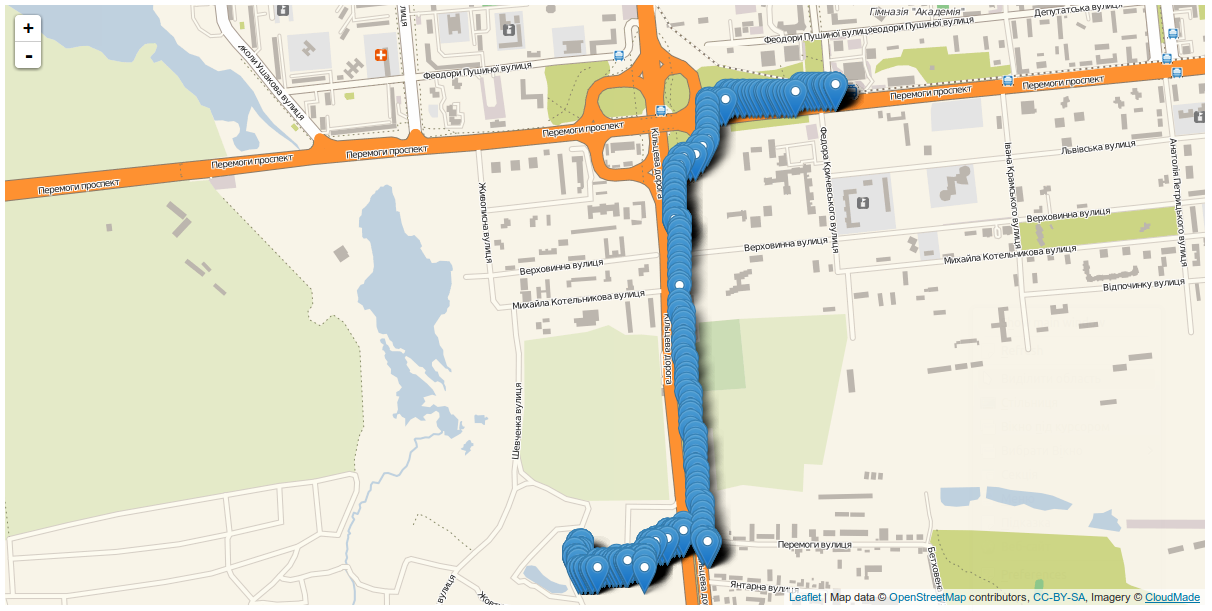
\includegraphics[scale=0.35]{images/results1.png}
	
	\vspace{2em}
	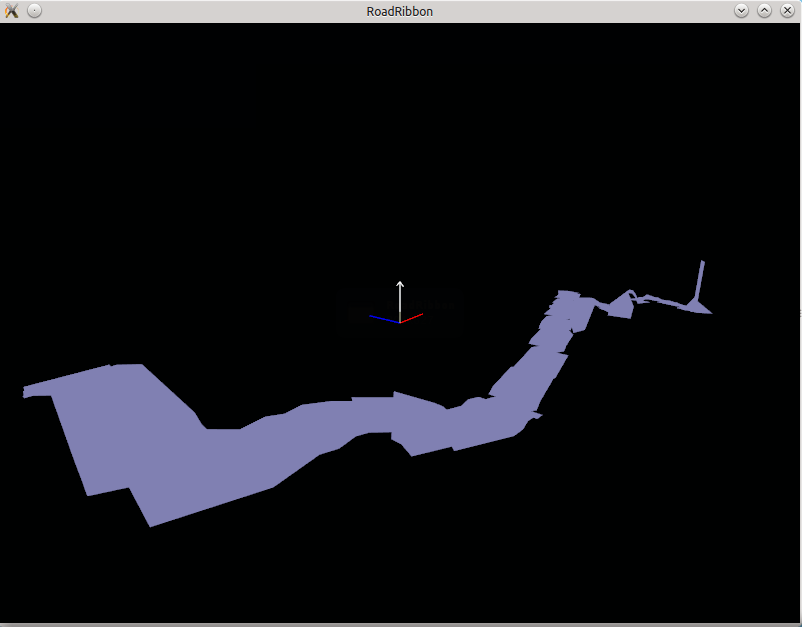
\includegraphics[scale=0.5]{images/results2.png}

  \newpage
  \section*{Висновки}
  \addcontentsline{toc}{section}{Висновки}

    Під час виконання роботи було проаналізовано існуючі системи та формати відстеження гео-позиції на планеті та висоти над рівнем моря у цій позиції за допомогою супутників мережі GPS.

    В рамках роботи було створено систему для відслідковування зміни гео-положення та запису пройденого маршруту у файл на смартфоні та систему візуалізації отриманих даних у вигляді тривимірної поверхні пройденого треку. Розроблені модулі показують сильні сторони мов програмування Java та C++, можливості платформ розробки Qt та Android, демонструють функціональну широту бібліотек SFML та OpenGL. Програмний код відповідає сучасним вимогам кодування та простий для розуміння.

    Розроблена система відкриває нові площини для досліджень. Показані ідеї можуть та будуть втілені в інших розробках в галузі гео-кодування та автомобільно-дорожніх системах, системах навігації та гео-інформаційних системах.

    \newpage
    \begin{appendices}

                \section{Охорона праці}

            \subsection{Загальні положення}

                Правила охорони праці при експлуатації електронно-обчислювальних машин (далі --- Правила) поширюються на всі підприємства, організації, юридичних осіб, незалежно від форми власності, відомчої належності, видів діяльності, і на фізичних осіб (які займаються підприємницькою діяльністю з правом наймання робочої сили), що здійснюють розробку, виробництво і використання електронно-обчислювальних машин і персональних комп'ютерів (далі - ЕОМ), чи виконують обслуговування, ремонт і налагодження ЕОМ.

                Правила встановлюють вимоги безпеки і санітарно-гігієнічні вимоги до устаткування робочих місць користувачів ЕОМ і працівників, що виконують обслуговування, ремонт і налагодження ЕОМ, відповідно до сучасного стану техніки і наукових досліджень у сфері безпечної організації робіт з експлуатації ЕОМ і з урахуванням положень міжнародних нормативно-правових актів з цих питань (директиви Ради Європейського союзу 90/270/ЄЕС, 89/391/ЄЕС, 89/654/ЄЕС, 89/655/ЄЕС, стандарти ISO, MPRII).

                Вимоги Правил не поширюються на:

                \begin{itemize}
                    \item комп'ютерні класи вищих і середніх навчальних закладів, майстерні професійно-технічних навчальних закладів;
                    \item робочі місця операторів ЕОМ, які використовуються у сфері керування й експлуатації атомних електростанцій;
                    \item робочі місця пілотів, чи водіїв-операторів транспортних засобів, обладнаних ЕОМ, ЕОМ у системах обробки даних на бортах засобів повідомлення й ЕОМ у складі машин і устаткування, що переміщується у процесі роботи;
                    \item так називані портативні системи обробки даних, якщо вони використовуються на робочому місці мінливо;
                    \item обчислювальні машинки (калькулятори), каси, які регіструють, і прилади з невеликими пристроями індикації чи даних результатів вимірів;
                    \item друкарські машинки класичної конструкції, обладнані відеотерміналом (так названі дисплейні друкарські машинки);
                    \item комп'ютерні ігрові автомати і системи обробки даних, призначені для суспільного користування;
                \end{itemize}

                Вимоги Правил є обов'язковими для всіх працівників при організації і виконанні робіт, пов'язаних з експлуатацією, обслуговуванням, налагодженням і ремонтом ЕОМ, а також при проектуванні і реконструкції підприємств, їхніх виробничих об'єктів, споруджень і робочих місць, обладнаних ЕОМ.

                Робочі місця повинні в повному обсязі задовольняти вимогам даних Правил.

                Власники, керівники служб і структурних підрозділів, безпосередні керівники робіт та інші посадові особи підприємств, фізичні особи, що займаються підприємницькою діяльністю з правом наймання робочої сили, забезпечують виконання даних Правил у межах покладених на них задач і функціональних обов'язків відповідно до чинного законодавства.

            \subsection{Вимоги до виробничих приміщень}

                Облаштованість робочих місць, обладнаних відеотерміналами, повинне забезпечувати:

                \begin{itemize}
                    \item належні умови освітлення приміщення і місця робітника, відсутність відблисків;
                    \item оптимальні параметри мікроклімату (температура, відносна вологість повітря, швидкість руху, рівень іонізації повітря);
                    \item належні ергономічні характеристики основних елементів робочого місця;
                \end{itemize}

                а також враховувати наступні небезпечні і шкідливі фактори:

                \begin{itemize}
                    \item наявність шуму і вібрації;
                    \item м'яке рентгенівське випромінювання;
                    \item електромагнітне випромінювання;
                    \item ультрафіолетове й інфрачервоне випромінювання;
                    \item електростатичне поле між екраном і оператором;
                    \item наявність пилу, озону, окислів азоту й іонізації.
                \end{itemize}

                Будинки і приміщення, у яких експлуатуються ЕОМ і відбувається їхнє обслуговування, налагодження і ремонт, повинні відповідати вимогам нормативно-технічної й експлуатаційної документації заводу-виробника ЕОМ, що діють, санітарних норм і правил, правил у сфері охорони праці і цих Правил.

                Робочі місця з відеотерміналами чи персональні ЕОМ у приміщеннях із джерелами шкідливих виробничих факторів повинні розміщатися в ізольованих кабінах з обладнаним повітрообміном.


                Стіни кабін виготовляються з непальних матеріалів. Допускається виготовляти їх зі скла і металевих конструкцій. Кабіна повинна мати оглядове вікно (вікна). Висота оглядового вікна повинна бути не менш 1.5 м, а відстань від підлоги не більш 0,8 м.

                Площа приміщень, у яких розміщують відеотермінали, визначають відповідно до діючих нормативних документів з розрахунку на одне робоче місце, обладнане відеотерміналом: площа -- не менш 6.0 м$^{2}$, обсяг -- не менш 20.0 м$^{3}$, з урахуванням максимальної кількості людей, що одночасно працюють у зміні.

                Стіни, стеля, підлога приміщень, у яких розміщені ЕОМ, повинні бути виготовлені з матеріалів, дозволених для оформлення приміщень органами державного санітарно-епідеміологічного нагляду.

                Заземлені конструкції, що знаходяться в приміщеннях (батареї опалення, водопровідні труби, кабелі з заземленим відкритим екраном і т.п.), повинні бути надійно захищені діелектричними щитками чи сітками від випадкового дотику.

                У приміщеннях з ЕОМ варто щодня робити вологе збирання.

                У приміщеннях з ЕОМ повинні знаходитися медичні аптечки першої допомоги.

                Приміщення з ЕОМ повинні бути оснащені переносними вуглекислотними вогнегасниками з розрахунку 2 шт. на кожні 20 м$^{2}$ площі приміщення з обліком гранично припустимих концентрацій вогнегасників відповідно до вимог Правил пожежної безпеки України. В інших приміщеннях допускається встановлювати теплові пожежні оповісники.

                Підходи до засобів пожежегасіння повинні бути вільні.

            \subsection{Санітарно-гігієнічні вимоги}

                Приміщення з ЕОМ повинні мати природне і штучне освітлення у відповідності зі Сніп II-4-79 «Природне і штучне освітлення».

                Природне світло повинне проникати через бічні світлові прорізи, зорієнтовані, як правило, на північ чи північний схід, і забезпечувати коефіцієнт освітленості (КЕО) не нижче 1,5\%.

                При виробничій необхідності допускається експлуатація ЕОМ у приміщеннях без природного освітлення за узгодженням з органами державного нагляду за охороною праці й органами санітарно-епідеміологічної служби.

                Вікна приміщень з відеотерміналами повинні мати регулювальні пристрої для відкривання, а також жалюзі,  штори, зовнішні козирки і т.п.

                Штучне освітлення приміщення з робочими місцями, обладнаними відеотерміналами ЕОМ загального і персонального користування, повинне бути обладнано системою загального рівномірного освітлення. У виробничих і адміністративно-суспільних приміщеннях, де переважає робота з документами, допускається застосування системи комбінованого освітлення (установка додатково до загального освітлення світильників місцевого освітлення).

                Загальне освітлення повинне бути виконане у виді суцільних чи переривчастих ліній світильників, розташовуваних збоку від робочих місць (переважно ліворуч) паралельно напрямку зору працівників. Допускається застосування світильників наступних класів світлорозподілу:

                \begin{itemize}
                    \item світильники прямого світла -- П;
                    \item переважно прямого світла -- Н;
                    \item переважно відбитого світла -- В.
                \end{itemize}

                При розташуванні відеотерміналів ЕОМ по периметрі приміщення лінії світильників штучного освітлення повинні розміщатися локально над робочими місцями.

                Для загального освітлення необхідно застосовувати світильники з розсіювачами і дзеркальними екранними відбивачами чи сітками, укомплектованими високочастотними регулюючими апаратами, (ВЧ ПРА). Застосування світильників без розсіювачів і екранних сіток забороняється.

                Як джерело світла при штучному освітленні повинні застосовуватися, як правило, люмінесцентні лампи типу ЛБ. При устаткуванні відбитого світла у виробничих і адміністративно-суспільних приміщеннях можуть застосовуватися метало-галогенові лампи потужністю до 250Вт. У світильниках місцевого освітлення допускається застосування ламп накалювання.

                Яскравість світильників загального освітлення в зоні кутів випромінювання від 500 до 900 по вертикалі в подовжній і поперечній площинах повинна складати не більш 200 кд/м$^{2}$, а захисний кут світильників повинний бути не більш 400.

                Коефіцієнт пульсації не повинний перевищувати 5\% і забезпечуватися застосуванням газорозрядних ламп у світильниках загального і місцевого освітлення.

                При відсутності світильників із ВЧ ПРА лампи багатолампових світильників чи розташовані поруч світильники загального освітлення необхідно підключати до різних фаз трифазної мережі.

                Рівень освітленості на робочому столі в зоні розміщення документів повинний бути в межах 300-500 лк. У випадку неможливості забезпечити системою загального освітлення даний рівень освітленості допускається застосування світильників місцевого освітлення; при цьому не повинно бути відблисків на поверхні екрана і збільшення освітленості екрана більш ніж 300 лк.

                Необхідно обмежувати відблиск шляхом правильного вибору типів світильників і розміщенням робочих місць щодо освітлення. При цьому яскравість відблисків на екрані відеотермінала не повинна  перевищувати 40 кд/м$^{2}$, яскравість стелі при застосуванні системи відбитого освітлення не повинна перевищувати 200 кд/м$^{2}$.

                Необхідно використовувати систему вимикачів, що дозволяє регулювати інтенсивність штучного освітлення в залежності від інтенсивності природного, а також висвітлювати тільки необхідні для роботи зони приміщення.

                Для забезпечення нормованих рівнів шуму у виробничих приміщеннях і на робочих місцях застосовуються шумопоглинальні засоби, вибір яких влаштовується спеціальними інженерно-акустичними розрахунками.

                Як засоби звукопоглинання повинні премінятися непальні чи важкозапалювані спеціальні перфоровані плити, панелі, мінеральна вата з максимальним коефіцієнтом звукопоглинання в межах частот 31,5 -- 8000 Гц, чи інші матеріали аналогічного призначення, дозволені органами державного нагляду для оформлення приміщень. Крім того, необхідно застосовувати підвісні стелі з аналогічними властивостями.

                Приміщення з ЕОМ повинні бути обладнані системами опалення, кондиціонування чи приточно-витяжною вентиляцією.

                Рівні електромагнітного випромінювання і магнітних полів повинні відповідати вимогам ДСТ 12.1.006 «ССБТ. Електромагнітні поля радіочастот. Припустимі рівні на робочих місцях і вимоги до проведення контролю» і СН № 3206-85 «Гранично припустимі рівні магнітних полів частотою 50 Гц».

                Рівні інфрачервоного випромінювання не повинні перевищувати граничних відповідно до ДСТ 12.1.005 і СН № 4088-86 з урахуванням площі опромінення тіла.

                Рівні ультрафіолетового випромінювання не повинні перевищувати припустимих відповідно до СН № 4557-88 «Санітарні норми ультрафіолетового випромінювання у виробничих приміщеннях».

                Гранично припустима напруженість електростатичного поля на робочих місцях не повинна перевищувати рівнів, приведених у ДСТ 12.1.045 «ССБТ. Електростатичні поля. Припустимі рівні на робочих місцях і вимоги до проведення контролю», СН № 1757-77 «Санітарно-гігієнічні норми припустимої напруженості електростатичного поля».

                Потужність експозиційної дози рентгенівського випромінювання на відстані 0,05 м від екрана і корпуса відеотермінала при будь-яких положеннях регулюючих пристроїв відповідно до Норм радіаційної безпеки України (НРБУ-97), затвердженими постановою державного санітарного Міністерства Охорони Здоров'я України від 18.08.97 № 58, не повинна перевищувати $7,74 \times 10-12$ А/кГ, що відповідає еквівалентній дозі 0.1 мбер/год (100 мкР/ч).

                Відповідно до ДСТ 12.1.005-88 вміст озону в повітрі робочої зони не повинен перевищувати 0.1 мг/м$^{3}$; зміст оксидів азоту -- 5 мг/м$^{3}$; зміст пилу -- 4 мг/м$^{3}$.

                При використанні одним працівником декількох відеотерміналів чи персональних ЕОМ санітарно-гігієнічні параметри виробничого середовища на робочому місці користувача повинні відповідати вищевказаним вимогам.

            \subsection{Вимоги електробезпеки}

                ЕОМ, периферійні пристрої ЕОМ і устаткування для обслуговування, ремонту і налагодження ЕОМ, інше устаткування (апарати керування, контрольно-вимірювальні прилади, світильники і т.п.), електропроводи і кабелі по виконанню і ступеню захисту повинні відповідати класу зони по ПУЕ, мати апаратуру захисту від струму короткого замикання й інших аварійних режимів.
                \linebreak\linebreak
                При монтажі й експлуатації ліній електромережі необхідно цілком виключити можливість виникнення електричного джерела запалення внаслідок короткого замикання і перевантаження проводів з легкозаймистою ізоляцією і, по можливості, перейти на непальну ізоляцію.

                При ремонті ліній електромережі шляхом зварювання, пайки з використанням відкритого вогню необхідно дотримуватися Правил пожежної безпеки Україні.

                Лінія електромережі для живлення ЕОМ, периферійних пристроїв ЕОМ і устаткування для обслуговування, ремонту і налагодження ЕОМ виповнюється як окрема групова трипроводна мережа, шляхом прокладання фазового, нульового робочого і нульового захисного провідників. Нульовий захисний провідник використовується для заземлення (занулення) електроприймачів.

                Використання нульового робочого провідника як нульового захисного провідника забороняється.

                Нульовий захисний провідник прокладається від стійки групового розподільного щита, розподільного пункту до розеток живлення.

                Не допускається підключення на щиті до одного контактного затиску нульового робочого і нульового захисного провідників.

                Площа перетину нульового робочого і нульового захисного провідників у груповій трипровідній мережі повинна бути не менше площі перетину фазового провідника. Усі провідники повинні відповідати номінальним параметрам мережі і навантаження, умовам навколишнього середовища, умовам розподілу провідників, температурному режиму і типам захисної апаратури, вимогам ПУЕ.

                У приміщенні, де одночасно експлуатується чи обслуговується більш п'яти персональних ЕОМ, на видному і доступному місці встановлюється аварійний резервний вимикач, що може цілком відключити електричне живлення приміщення, за винятком освітлення.

                ЕОМ, периферійні пристрої ЕОМ і устаткування для обслуговування, ремонту і налагодження ЕОМ повинні підключатися до електромережі тільки за допомогою справних штепсельних з'єднань і електророзеток фабричного виготовлення.

                Штепсельні з'єднання і електророзетки крім контактів фазового і нульового робочого провідників повинні мати спеціальні контакти для підключення нульового захисного провідника. Конструкція їх повинна бути такою, щоб приєднання нульового захисного провідника відбувалося раніше, ніж приєднання фазового і нульового робочого провідників. Порядок роз'єднання при відключенні повинний бути зворотним. Необхідно виключити можливість з'єднання контактів фазових провідників з контактами нульового захисного провідника.

                Неприпустиме підключення ЕОМ, периферійних пристроїв ЕОМ і устаткування для обслуговування, ремонту і налагодження ЕОМ до звичайної двохпровідної електромережі, у тому числі -- з використанням перехідних пристроїв.

                Електромережі штепсельних з'єднань і електророзеток для живлення персональних ЕОМ, периферійних пристроїв ЕОМ і устаткування для обслуговування, ремонту і налагодження ЕОМ варто виконувати за магістральною схемою, по 3 -- 6 з'єднань чи електророзеток в одному ланцюзі.

                Штепсельні з'єднання і електророзетки для напруги 12 В и 36 В по своїй конструкції повинні відрізнятися від штепсельних з'єднань для напруги 127 В и 220 В.

                Штепсельні з'єднання і електророзетки, розраховані на напругу 12В і 36В, мають бути пофарбовані в колір, що візуально значно відрізняється від кольору штепсельних з'єднань, розрахованих на напругу 127 В и 220 В.

                Індивідуальні і групові штепсельні з'єднання і електророзетки необхідно монтувати на непальних чи важкозапалюваних пластинах з урахуванням вимог ПУЕ і Правил пожежної безпеки України.

                Для підключення переносної електроапаратури застосовуються гнучкі проводи в надійній ізоляції.

                Тимчасова електропроводка від переносних приладів до джерел живлення виконується  найкоротшим шляхом, щоб уникнути заплутування проводів у конструкціях машин, приладах і меблях. Нарощувати провід можна тільки шляхом пайки з наступним старанним ізолюванням місць з'єднання.

                Неприпустимим є:

                \begin{itemize}
                    \item експлуатація кабелів і проводів з ушкодженою чи втратившою захисні властивості за час експлуатації ізоляцією; залишення під напругою кабелів і проводів з неізольованими провідниками;
                    \item застосування саморобних подовжувачів, що не відповідають вимогам ПУЕ до переносних електропроводів;
                    \item застосування для опалення приміщення нестандартного (саморобного) електронагрівального устаткування чи ламп накалювання;
                    \item користування ушкодженими розетками, розвідними і з'єднуючими коробками, вимикачами й іншими електроприладами, а також лампами, скло яких має сліди затемнення і здуття;
                    \item підвішування світильників безпосередньо на струмоведучих проводах, обгортання електроламп і світильників папером, тканиною й іншими пальними матеріалами, експлуатація їх зі знятими ковпаками (розсіювачами);
                    \item використання електроапаратури і приладів в умовах, що не відповідають вказівкам (рекомендаціям) підприємств-виготовлювачів.
                \end{itemize}

            \subsection{Вимоги до устаткування}

                Відеотермінали, ЕОМ, ПЕВМ, спеціальні периферійні пристрої ЕОМ і устаткування для обслуговування, ремонту і налагодження ЕОМ повинні відповідати діючим в Україні стандартам, нормативним актам про охорону праці і цих Правил. Відеотермінали, ЕОМ, ПЕВМ, спеціальні периферійні пристрої ЕОМ іноземного виробництва, крім того, повинні відповідати вимогам національних стандартів держав-виробників і мати відповідні відмітки на корпусі, у паспорті чи іншій експлуатаційній документації.

                Забороняється використання для виробничих потреб нових відеотерміналів, ЕОМ, ПЕВМ, спеціальних периферійних пристроїв ЕОМ і устаткування для обслуговування, ремонту і налагодження ЕОМ, що підлягають обов'язковій сертифікації в Україні, чи в стандартах, які вимагають забезпечення безпеки праці, життя і здоров'я людей, без наявності виданого в Україні згідно державній системі сертифікації Укрсепро, що засвідчує їхню відповідність обов'язковим вимогам.

                Прийняття в експлуатацію зазначеного устаткування повинне здійснюватися тільки при наявності в комплекті з ним паспорта, інструкції чи іншої експлуатаційної документації, переведеної на українську чи російську мови.

                При наявності відхилень від вимог нормативної документації можливість використання устаткування повинна бути передбачена у контракті на постачання, погоджена з Держнадзором по охороні праці, Держстандартом і організацією-замовником. Копії погоджень і сертифікати повинні бути залучені до паспорта чи іншої експлуатаційної документації устаткування.

                По способу захисту людини від поразки електричним струмом відеотермінали, ЕОМ, периферійні пристрої ЕОМ і устаткування для обслуговування, ремонту і налагодження ЕОМ повинні відповідати I класу захисту відповідно ДО ДЕРЖСТАНДАРТУ і ДСТ 25861-83 «Машини обчислювальні і системи обробки даних. Вимоги електричної і механічної безпеки і методи іспитів» чи повинні бути заземлені відповідно до ДНАОП 0.00-1.21-98.

                Недопустимо використання клем функціонального заземлення для підключення захисного заземлення.

                Відеотермінали повинні відповідати наступним критеріям. Яскравість від 35 до 120 кд/м2. Зовнішня освітленість від 100 до 250 лк. Нерівномірність яскравості в робочій зоні екрана не більш 1,7:1. Відхилення форми робочої зони від прямокутності по горизонталі і вертикалі не більш 2\%, а по діагоналі не більше 4\% відношення суми коротких сторін до суми довгих. Різниця довжин рядків чи стовпців не більше 2\% середнього значення. Розмір мінімального елемента зображення (піксела) для монохромних зображень 0,3 мм.

                Вимоги щодо припустимих значень неіонізуючого електромагнітного випромінювання:

                \begin{itemize}
                    \item напруженість електромагнітного поля на відстані 50 див навколо ВДТ по електричної складової не повинна перевищувати: у діапазоні частот 5 кгц -- 2 кгц 25 В/м, у діапазоні 2 кгц -- 400 кГц 2.5 В/м;
                    \item щільність магнітного потоку не повинна перевищувати: у діапазоні частот 5 кгц -- 2 кгц 250 нтл, у діапазоні 2 кгц -- 400 кгц 25 нтл;
                    \item поверхневий електростатичний потенціал не повинний перевищувати 500 В;
                    \item потужність дози рентгенівського випромінювання на відстані 5 див від екрана й інших поверхонь ВДТ не повинна перевищувати 100 мкр/рік.
                \end{itemize}

                Вимоги до клавіатури:

                \begin{itemize}
                    \item виконання клавіатури у виді окремого пристрою з можливістю вільного переміщення;
                    \item наявність опорного пристрою, що надає можливість змінювати кут нахилу клавіатури в межах від 50 до 150 і виготовленого з матеріалу з великим коефіцієнтом тертя, що перешкоджає його переміщенню;
                    \item висота на рівні переднього ряду не більш 15 мм;
                    \item виділення кольором і місцем розташування окремих груп клавіш;
                    \item наявність поглиблень у середині клавіш;
                    \item однаковий хід усіх клавіш з мінімальним опором натиску 0,25 Н и максимальним не більш 1,5 Н;
                    \item виділення кольором на клавішах символів різних алфавітів (англійського, українського чи росіянина).
                \end{itemize}

            \subsection{Вимоги до розміщення устаткування й організації робочих місць}

                Організація робочого місця користувача відеотермінала й ЕОМ повинна забезпечувати відповідність всіх елементів робочого місця і їхнє розташування ергономічним вимогам ДСТ 12.2.032 «ССБТ. Робоче місце при виконанні робіт сидячи. Загальні ергономічні вимоги»; характеру й особливостям трудової діяльності.

                Площа, виділена для одного робочого місця з відеотерміналом чи персональною ЕОМ, повинна складати не менш 6 м$^{2}$, а обсяг -- не менше 20 м$^{3}$.

                Робочі місця з відеотерміналами щодо світлових прорізів повинні розміщатися так, щоб природне світло падало збоку, переважно ліворуч.

                При розміщенні робочих місць з відеотерміналами і персональними ЕОМ необхідно слідувати таким вимогам:

                \begin{itemize}
                    \item робочі місця з видеотреміналами і персональними ЕОМ розміщаються на відстані не менш 1 м від стін зі світловими прорізами;
                    \item відстань між бічними поверхнями відеотерміналів повинна бути не меншою за 1,2 м;
                    \item відстань між тильною поверхнею одного відеотермінала й екраном іншого не повинна бути менше ніж 2,5 м;
                    \item прохід між рядами робочих місць повинний бути не менш 1 м.
                \end{itemize}

                Конструкція робочого місця користувача відеотерміналом (при роботі сидячи) повинна забезпечувати підтримку оптимальної робочої пози з такими ергономічними характеристиками: стопи ніг -- на підлозі чи на підставці для ніг; стегна -- у горизонтальній площині; передпліччя -- вертикальні; лікті -- під кутом 70-900 до вертикальної площини; зап'ястя зігнуті під кутом не більш 200 щодо горизонтальної площини, нахил голови -- 15-200 щодо вертикальної площини.

                Якщо користування відеотерміналом і персональною ЕОМ є основним видом діяльності, то зазначене устаткування розміщується на основному робочому столі, як правило, з лівої сторони.

                Якщо використання відеотермінала і персональної ЕОМ є періодичним, то устаткування, як правило, розміщується на приставному столі, переважно з лівої сторони від основного робочого столу. Кут між подовжніми осями основного і приставного столів повинний бути 90-1400.

                Якщо використання відеотермінала і персональної ЕОМ є періодичним, то допускається обладнати в приміщенні, що відповідає вимогам, окремі робочі місця колективного користування з відеотерміналом і персональною ЕОМ.

                Висота робочої поверхні столу для відеотермінала повинна знаходитися в межах 680-800 мм.

                Розміри столу, що рекомендуються: висота - 725 мм, ширина - 600-1400 мм, глибина - 800-1000 мм.

                Робочий стіл для відеотермінала повинний мати простір для ніг висотою не менш 600 мм, шириною не менш 500 мм, глибиною на рівні колін не менш 450 мм, на рівні витягнутої ноги -- не менш 650 мм.

                Робочий стіл для відеотермінала, як правило, повинний бути обладнаний підставкою для одного шириною не менш 300 мм і глибиною не менш 400 мм, з можливістю регулювання по висоті в межах 150 мм і кута нахилу опорної поверхні -- у межах 200. Підставка повинна мати рифлену поверхню і бортик на передньому краї висотою 10 мм. Робоче сидіння (стілець, крісло) користувача відеотермінала і персональної ЕОМ повинне мати наступні основні елементи: сидіння, спинку і стаціонарні чи знімні підлокітники.

                У конструкцію сидіння можуть бути введені додаткові елементи, що є не обов'язковими: підголівник і підставка для ніг.

                Робоче сидіння користувача відеотермінала і персональної ЕОМ повинне бути підйомно-поворотним, регульованим по висоті, куту нахилу сидіння і спинки, по відстані спинки від переднього краю сидіння, по висоті підлокітників.

                Регулювання кожного параметра повинне бути незалежним, мати надійну фіксацію.

                Хід східчастого регулювання елементів сидіння повинний складати для лінійних розмірів 15-20 мм, для кутових -- 2-50.

                Усили при регулюванні не повинні перевищувати 20 Н.

                Ширина і глибина сидіння не повинна бути менше за 400 мм. Висота поверхні сидіння повинна регулюватися в межах 400-500 мм, а кут нахилу поверхні -- від 150 уперед до 50 назад.

                Поверхня сидіння повинна бути плоскою, передній край -- закругленим.

                Висота с пинки сидіння повинна складати 300..200 мм, ширина -- не менш 380 мм, радіус кривизни в горизонтальній площині -- 400 мм. Кут нахилу спинки повинний регулюватися в межах 0-300 щодо вертикального положення. Відстань від спинки до переднього краю сидіння повинна регулюватися в межах 260-400 мм.

                Для зменшення статичної напруги м'язів рук необхідно застосовувати стаціонарні чи знімні підлокітники довжиною не менш 250 мм, шириною -- 50-70 мм, що регулюються по висоті над сидінням у межах 230-330 мм і по відстані між підлокітниками в межах 350-500 мм.

                Поверхня сидіння, спинки і підлокітників повинна бути напівм'якою, з декількома, що не електризуються, повітронепроникними покриттями і забезпечувати можливість чищення від бруду.

                Екран відеотермінала і клавіатура повинні розташовуватися на оптимальній відстані від очей користувача, але не ближче 600 мм, з урахуванням розміру алфавітно-цифрових знаків і символів.

                Відстань від екрана до очей працівника повинна складати при розмірі екрана по діагоналі 35\ensuremath{\backslash}38 див (14''/15'') -- 600-700 мм, 43 див (17'') -- 700-800 мм, 48 див (19{``}) -- 800-900 мм, 53 див (21'') -- 900-1000 мм.

                Розташування екрана відеотермінала повинне забезпечувати зручність зорового спостереження у вертикальній площині під кутом $30^{\circ}$ від напрямку погляду працівника.

                Клавіатуру варто розміщати на поверхні столу чи на спеціальній, регульованій по висоті, робочій поверхні, окремо від столу на відстані 100-300 мм від краю, найближчого до працівника. Кут нахилу клавіатури повинний бути в межах 5-150.

                Робоче місце з відеотерміналом варто обладнати легко переміщуваним пюпітром для документів.

                Пюпітр для документів повинний бути рухливим і установлюватися вертикально (чи з нахилом) на тому ж рівні і відстані від очей користувача ЕОМ, що і відеотермінал.

                Розміщення принтера чи іншого пристрою вводу-виводу інформації на робочому місці повинне забезпечувати гарну видимість екрана відеотермінала, зручність ручного керування пристроєм вводу-виводу інформації в зоні досяжності поля: по висоті 900-1300 мм, по глибині 400-500 мм.

                Під матричні принтери варто підкладати вібраційні коврики для гасіння вібрації і шуму.

                При необхідності високої концентрації уваги під час виконання робіт з високим рівнем напруженості суміжні робочі місця з відеотерміналами і персональними ЕОМ необхідно відокремлювати друг від друга перегородками висотою 1,5 -- 2 м.

                Організація робочого місця, яка передбачає використання ЕОМ для керування технологічним устаткуванням (верстати з програмним керуванням, роботоризировані технологічні комплекси, устаткування для гнучкого автоматизованого виробництва тощо), повинна передбачати:

                \begin{itemize}
                    \item достатній простір для людини-оператора;
                    \item вільну досяжність органів ручного керування в зоні поля: відстань по висоті -- 900-1330 мм, по глибині -- 400-500 мм;
                    \item розташування екрана відеотермінала в робочій зоні, що забезпечує зручність зорового спостереження у вертикальній площині під кутом $30^{\circ}$ від напрямку погляду оператора, а також зручність користування відеотерміналом при коректуванні керуючих програм одночасно з виконанням основних виробничих операцій;
                    \item можливість повороту екрана відеотермінала навколо горизонтальної і вертикальної осей.
                \end{itemize}

                Вимоги до безпеки при експлуатації, обслуговуванні, ремонті і налагодженні ЕОМ

            \subsection{Вимоги безпеки при експлуатації ЕОМ}

                Користувачі ЕОМ повинні стежити за тим, щоб відеотермінали, ЕОМ, периферійні пристрої ЕОМ і устаткування для обслуговування, ремонту і налагодження ЕОМ були справними і пройшли іспит відповідно до діючого законодавства.

                Щодня перед початком роботи необхідно проводити очищення екрана відеотермінала від пилу й інших забруднень.

                При виконанні робіт на ЕОМ необхідно дотримувати режими праці і відпочинку, описані в наступному підрозділі.

                Після закінчення роботи відеотермінал і персональна ЕОМ повинні бути відключені від електричної мережі.

                При виникненні аварійної ситуації необхідно негайно відключити відеотермінал і ЕОМ від електричної мережі.

                При необхідності для захисту від електромагнітних, електростатичних і інших полів можуть застосовуватися спеціальні технічні засоби, що мають відповідний сертифікат чи санітарно-гігієнічний висновок акредитованих органів щодо їхніх захисних властивостей.

                Неприпустимо:

                \begin{itemize}
                    \item обслуговування, ремонт і налагодження ЕОМ безпосередньо на робочому місці користувача ЕОМ;
                    \item збереження біля відеотерміналів і ЕОМ папера, дискет, інших носіїв інформації, запасних блоків, деталей і т.п., якщо вони не використовуються для поточної роботи;
                    \item відключення захисних пристроїв, самовільна зміна конструкції і складу ЕОМ, устаткування, а також їхнє технічне налагодження;
                    \item робота з відеотерміналами, у яких при роботі виникають нехарактерні сигнали, нестабільне зображення на екрані і т.п.;
                    \item робота на матричному принтері зі знятою верхньою кришкою.
                \end{itemize}

            \subsection{Вимоги безпеки при обслуговуванні, ремонті і налагодженні ЕОМ}

                Монтаж, обслуговування, ремонт і налагодження ЕОМ, заміна деталей, пристроїв, блоків повинні здійснюватися тільки при цілком відключеному живленні.

                Забороняється з'єднувати і роз'єднувати кабелі при підключеній напрузі.

                У тих випадках, коли монтаж, обслуговування, ремонт і налагодження ЕОМ, її пристроїв, блоків при відключеному живленні неможливі, виконання цих робіт допускається при дотриманні наступних вимог:

                \begin{itemize}
                    \item устаткування, допоміжна апаратура і прилади повинні бути заземлені;
                    \item роботи виконуються не менш чим двома працівниками;
                    \item працівники повинні виконувати роботу інструментом з ізольованими ручками, на діелектричних ковриках, чи бути в діелектричних калошах.
                \end{itemize}

                Засоби захисту й інструмент необхідно щораз перед застосуванням оглянути і при виявленні несправностей негайно замінити.

                Користування несправними захисними засобами й інструментом неприпустимо. При виконанні ремонтних робіт варто користатися електроінструментом, напруга живлення якого не перевищує 36 В.

                Людям, що виконують ремонтні роботи, забороняється працювати з надягнутим на руку ручним годинником, що має металевий браслет.

                Працівникам, що виконують обслуговування, ремонт і налагодження ЕОМ, не дозволяється:

                \begin{itemize}
                    \item працювати поблизу відкритих струмоведучих частин;
                    \item залишати без догляду включене в мережу живлення устаткування, прилади, використовувані при проведенні робіт;
                    \item залишати на устаткуванні і приладах запобіжники, з'єднувачі, проводи, залишки флюсу, припою і т.п.;
                    \item розміщати на одному робочому столі (місці) два чи більш включених у мережу живлення відеотерміналів зі знятими футлярами;
                    \item робити всередині відеотермінала операції, виконувані тільки двома руками, без попереднього відключення відеотермінала від мережі живлення і зняття залишкових зарядів з конденсаторів, фільтра-випрямителя та інших анодів кінескопа.
                \end{itemize}

            \subsection{Режим праці і відпочинку}

                Режим праці й відпочинку працюючих з ЕОМ визначається в залежності від виконуваної роботи відповідно до ДСанПіН 3.3.2-007-98.

                Залучення жінок до роботи в нічний час не допускається, за винятком випадків, обумовлених статтею 175 Кодексу законів про працю України.

                Якщо виробляється психологічне розвантаження працівників, що виконують роботи з застосуванням ЕОМ, вона повинна вироблятися в спеціально обладнаних приміщеннях (кімнатах психологічного розвантаження) під час регламентованих перерв чи наприкінці робочого дня -- відповідно до методики проведення психофізіологічного розвантаження, викладеної в додатку 9  до ДСанПіН 3.3.2-007-98.

            \subsection{Вимоги до виробничого персоналу}

                Усі працівники, що виконують роботи, зв'язані з експлуатацією, обслуговуванням, налагодженням і ремонтом ЕОМ, підлягають обов'язковим медичним оглядам -- попередньому при оформленні на роботу і періодичним у плині трудової діяльності -- у порядку, з періодичністю і медичними протипоказаннями відповідно до Положення про медичні огляди працівників визначених категорій, затвердженим наказом Міністерства Охорони Здоров'я України 31 березня 1994 року №45 і зареєстрованим у Міністерстві юстиції України 21.06.94 за №136/345, і ДСанПіН 3.3.2-007-98.

                Посадові особи і фахівці, інші працівники підприємств, зайняті організацією і виконанням робіт, зв'язаних з експлуатацією, профілактичним обслуговуванням, налагодженням і ремонтом ЕОМ, проходять підготовку (підвищення кваліфікації), перевірку знань по охороні праці, питань пожежної безпеки, а також інструктажі у порядку, передбаченому Типовим положенням про навчання з питань охорони праці, затвердженим наказом Держнадзору з охорони праці 17.02.99 № 27, зареєстрованим у Міністерстві юстиції України 21.04.99 за №248/3541, Типовим положенням про спеціальне навчання, інструктажі і перевірку знань з питань пожежної безпеки на підприємствах, у заснуваннях і організаціях України і Переліком посад, при призначенні на які працівники зобов'язані проходити навчання і перевірку знань з питань пожежної безпеки, і порядком її організації, затвердженими наказом МВС України від 17.11.94 № 628, зареєстрованим у Міністерстві юстиції України 22.12.94 за №307/517.

                До роботи безпосередньо на ЕОМ допускаються працівники, що не мають медичних протипоказань.

                Працівники, що виконують роботи з профілактичного обслуговування, налагодженню і ремонту ЕОМ при включеному живленні і при інших роботах, передбачених Переліком робіт з підвищеною небезпекою, затвердженим наказом Держнагляду з охорони праці 30.11.93 №123, зареєстрованим у Міністерстві юстиції України 23.12.93 за №196, зобов'язані проходити попереднє спеціальне навчання й один раз у рік перевірку знань відповідних нормативних актів по охороні праці.

                Допуск до роботи працівників, що не пройшли у встановленому порядку навчання, інструктаж і перевірку знань по охороні праці і пожежній безпеці забороняється.

                Забороняється допускати людей молодше 18 років до самостійних робіт в електроустановках і на електроустаткуванні при їхньому профілактичному обслуговуванні, налагодженні, ремонті ЕОМ і інших роботах, передбачених Переліком важких робіт і робіт зі шкідливими і небезпечними умовами праці, на яких забороняється застосування праці неповнолітніх, затвердженим наказом Міністерства охорони здоров'я України 31.03.94 №46, зареєстрованим у міністерстві юстиції України 28.04.94 за №176/385.

                До робіт по обслуговуванню, налагодженню і ремонту ЕОМ допускаються працівники, що мають кваліфікаційну групу з електробезпеки не нижче ІІІ.

                Працівники, що виконують роботи по експлуатації, обслуговуванню, налагодженню і ремонту ЕОМ, у відповідності зі статтею 10 Закону України «Про охорону праці» забезпечуються належними засобами індивідуального захисту відповідно до діючого законодавства.

            \subsection{Обов'язки, права і відповідальність за порушення правил}

                Обов'язки і права власника і працівника визначені чинним законодавством України.

                Відповідно до Закону України «Про охорону праці» власник:

                \begin{itemize}
                    \item вживає необхідні заходи для того, щоб робочі місця і засоби виробництва в плині всього часу їхнього використання підтримувались у справному і безпечному стані;
                    \item проводить відповідні навчання й інструктажі з працівниками;
                    \item проводить атестацію робочих місць для оцінки умов праці;
                    \item організовує роботу таким чином, щоб повсякденна робота з відеотерміналами переривалася паузами чи іншою діяльністю, яка знижує навантаження;
                    \item організовує проведення обстеження зору працівника окулістом.
                \end{itemize}

                Працівник має право:

                \begin{itemize}
                    \item на відповідне дослідження очей і зору людиною потрібної кваліфікації;
                    \item на одержання за рахунок власника індивідуальних засобів захисту;
                    \item на інформацію з усіх важливих питань, що стосуються його здоров'я і безпеки, пов'язану з перебуванням на робочому місці.
                    \item Відповідно до Закону України «Про охорону праці» працівник зобов'язаний:
                    \item знати і виконувати вимоги нормативних актів про охорону праці;
                    \item використовувати засоби колективного й індивідуального захисту;
                    \item виконувати обов'язки по охороні праці, передбачені колективним договором;
                    \item не відключати захисні пристрої, не робити самовільних змін конструкції і складу устаткування чи його технічного налагодження.
                \end{itemize}

                Власники, керівники служб і структурних підрозділів, і інші посадові особи підприємств, фізичні особи, що займаються підприємницькою діяльністю з правом наймання робочої сили, працівники несуть відповідальність за виконання вимог даних Правил у межах покладених на них завдань і функціональних обов'язків відповідно до діючого законодавства.

                За безпеку експлуатації, обслуговування, ремонту і налагодження ЕОМ, а також за відповідність устаткування, виробничих приміщень, робочих місць даним Правилам відповідає власник.

                Працівники, винні в порушенні цих Правил, несуть дисциплінарну, адміністративну, матеріальну і кримінальну відповідальність відповідно до діючого законодавства.

    \end{appendices}

\newpage

\bibliographystyle{gost2008}
\renewcommand\bibname{Використана література}
\bibliography{literature.bib}

\end{document}